%% Le lingue utilizzate, che verranno passate come opzioni al pacchetto babel. Come sempre, l'ultima indicata sarà quella primaria.
%% Se si utilizzano una o più lingue diverse da "italian" o "english", leggere le istruzioni in fondo.
\def\thudbabelopt{english}
%% Valori ammessi per target: bach (tesi triennale), mst (tesi magistrale), phd (tesi di dottorato).
%% Valori ammessi per aauheader: '' (vuoto -> nessun header Alpen Adria Univeristat), aics (Department of Artificial Intelligence and Cybersecurity), informatics (Department of Informatics Systems). Il nome del dipartimento è allineato con la versione inglese del logo UniUD.
%% Valori ammessi per style: '' (vuoto -> stile moderno), old (stile tradizionale).
\documentclass[target=bach,aauheader=,style=]{thud}

%% --- Informazioni sulla tesi ---
%% Per tutti i tipi di tesi
% Scommentare quello di interesse, o mettete quello che vi pare
\course{Informatica}
%\course{Internet of Things, Big Data e Web}
%\course{Matematica}
%\course{Comunicazione Multimediale e Tecnologie dell'Informazione}
\title{Automatic Nuclei Segmentation and Counting in Histopathology Images with U-Net}
\author{Pantanali Riccardo}
\supervisor{Prof.\ Della Mea Vincenzo}
\cosupervisor{Dott.ssa \ Teresa Pace}
\tutor{Guido Necchi}
%% Campi obbligatori: \title, \author e \course.
%% Altri campi disponibili: \reviewer, \tutor, \chair, \date (anno accademico, calcolato in automatico), \rights
%% Con \supervisor, \cosupervisor, \reviewer e \tutor si possono indicare più nomi separati da \and.
%% Per le sole tesi di dottorato:
\phdnumber{313}
\cycle{XXVIII}
\contacts{Via della Sintassi Astratta, 0/1\\65536 Gigatera --- Italia\\+39 0123 456789\\\texttt{http://www.example.com}\\\texttt{inbox@example.com}}

%% --- Pacchetti consigliati ---
%% pdfx: per generare il PDF/A per l'archiviazione. Necessario solo per la versione finale
\usepackage[a-1b]{pdfx}
%% hyperref: Regola le impostazioni della creazione del PDF... più tante altre cose. Ricordarsi di usare l'opzione pdfa.
\usepackage[pdfa]{hyperref}
\usepackage{tikz}
\usepackage{subcaption}
\usepackage{amsmath, amssymb,subcaption}
\usepackage{float}
\newlength{\colsep}
\setlength{\colsep}{4.2cm}
\usepackage{graphicx}
\usepackage{booktabs}
\usetikzlibrary{backgrounds}
\usetikzlibrary{calc,positioning, fit}
%% tocbibind: Inserisce nell'indice anche la lista delle figure, la bibliografia, ecc.

%% --- Stili di pagina disponibili (comando \pagestyle) ---
%% sfbig (predefinito): Apertura delle parti e dei capitoli col numero grande; titoli delle parti e dei capitoli e intestazioni di pagina in sans serif.
%% big: Come "sfbig", solo serif.
%% plain: Apertura delle parti e dei capitoli tradizionali di LaTeX; intestazioni di pagina come "big".

\begin{document}
\maketitle

%% Dedica (opzionale)
\begin{dedication}
	Al mio cane,\par per avermi ascoltato mentre ripassavo le lezioni.
\end{dedication}

%% Ringraziamenti (opzionali)
\acknowledgements
Sed vel lorem a arcu faucibus aliquet eu semper tortor. Aliquam dolor lacus, semper vitae ligula sed, blandit iaculis leo. Nam pharetra lobortis leo nec auctor. Pellentesque habitant morbi tristique senectus et netus et malesuada fames ac turpis egestas. Fusce ac risus pulvinar, congue eros non, interdum metus. Mauris tincidunt neque et aliquam imperdiet. Aenean ac tellus id nibh pellentesque pulvinar ut eu lacus. Proin tempor facilisis tortor, et hendrerit purus commodo laoreet. Quisque sed augue id ligula consectetur adipiscing. Vestibulum libero metus, lacinia ac vestibulum eu, varius non arcu. Nam et gravida velit.

%% Sommario (opzionale)
%\abstract

%% Indice
\tableofcontents

%% Lista delle tabelle (se presenti)
%\listoftables

%% Lista delle figure (se presenti)
\listoffigures

%% Corpo principale del documento
\mainmatter

%% Parte
%% La suddivisione in parti è opzionale; solitamente sono sufficienti i capitoli.
%\part{Parte}

%% Capitolo
\chapter{Introduction}
\label{sec:introduction}
Histopathology is the gold standard for cancer diagnosis in which tissue biopsies are stained and examined under the microscope by pathologists to determine the presence and extent of disease. Among these, the morphology, density and spatial distribution of cell nuclei, is of paramount importance to the diagnosis and prognosis. However, manual assessment is laborious, subjective and suffers from inter-observer variation, which drives the need for an automatic computer aided mechanism for segmentation and analysis of nuclei.
Deep learning in recent years has been considered a breakthrough technology in medical image analysis, achieving extraordinary performance in different tasks ranging from tumor detection, grading and quantification of biomarkers. Convolutional Neural Networks (CNNs) and their variant U-Net have emerged as the de facto method for biomedical image segmentation, achieving the reliable performance even under the presence of challenging imaging conditions. Building on these advancements, dedicated architectures, e.g. HoVer-Net \cite{graham2019hovernet}, have been introduced to separate clustered or overlapping nuclei through a simultaneous prediction of segment masks and distance maps.
Nevertheless, some challenging problems are left open. The publiavailable nuclei datasets are not only small, but also of a diverse quality, and containing the incomplete and noisy annotations. Furthermore, many nucleus are closely spaced, partly occluded or weakly stained and therefore especially difficult to separate. These constraints create major barriers to building trustworthy models for clinical use.
In this work, we consider the problem of segmenting and counting \textbf{neoplastic nuclei} in histopathology images. Unlike multi-class methods that target at classifying all nuclear subtypes, we are particularly interested in the classification of malignant nucleus since they are more relevant for cancer diagnosis and progression. This study is built upon the widely-used PanNuke dataset \cite{gamper2019pannuke,gamper2020pannuke} with instance-level nuclear annotations on multiple tissue types.

To address the segmentation and counting problem, we introduce a U-Net model with two task-specific heads: a segmentation head that produces a three-channel representation (\textit{body}, \textit{background}, \textit{border}), and a regression head that estimates horizontal and vertical distance maps of nuclei. This multi-head architecture allows the model to simultaneously learn categorical and geometric features, which is deeper and helps separate touching nuclei and robust counting.
We Also explore the impact of various image preprocessing modalities (RGB, hematoxylin-extracted H\&E, blue colormap, grayscale) on the model performance. This investigation seeks to clarify the role that color and intensity information plays in the segmentation and counting of neoplastic nuclei.

\section{Problem Definition and Objectives}
The objective of this work is to design a deep learning based framework for the segmentation and counting of the neoplastic nuclei in histopathology images. Specifically, we aim to:
\begin{enumerate}
\item Develop a pre-processing pipeline that preprocesses the PanNuke instance annotations into binary masks and distance maps for training.
\item Develop and train a multi-head U-Net model to predict both the segmentation masks and horizontal/vertical distance maps simultaneously.
\item Analyze how well the model generalizes across different input representations (RGB, Hematoxylin, Blue, Grayscale).
\item Show results in terms of both segmentation (Dice, IoU, AJI, PQ) and counting (MAE, $R^2$, Pearson correlation) metrics.
\item Inspect the error distribution between the categories of size and density of nuclear morphology to gain insight into the model behavior and the challenging cases.
\end{enumerate}

\section{Structure of the Thesis}
The rest of this thesis is structured as follows:
\begin{itemize}
\item \textbf{Chapter 2 (Theoretical Aspects)} provides the theoretical background underlying this work, including fundamentals of deep learning, convolutional neural networks, and related approaches for biomedical image segmentation and nuclei instance analysis.
\item \textbf{Chapter 3 (Dataset)} Presents the PanNuke dataset, followed by its creation process, class distribution, and the statistics related to our study.
\item \textbf{Chapter 4 (Method)} Defines the whole pipeline by preprocessing, proposed multi-head U-Net architecture, losses, training strategy, and post-processing steps.
\item \textbf{Chapter 5 (Results)} Presents the experimental results including the comparison of different preprocessing options as well as an investigation of the segmentation and counting quality.
\item \textbf{Chapter 6} (\textbf{Discussion and Conclusion}) Summarizes key findings, discusses limitations and suggests potential future research directions.
\end{itemize}
\chapter{Theoretical aspect}
\label{sec:theory}
This chapter introduces the theoretical foundations required to understand the methods and experiments presented in this thesis. 
We begin with an overview of digital histopathology, highlighting the role of hematoxylin and eosin (H\&E) staining in emphasizing nuclear morphology and motivating the use of color deconvolution techniques to isolate relevant channels such as hematoxylin, blue, and grayscale representations. 
We then provide the necessary background on convolutional neural networks (CNNs) and encoder-decoder architectures, with particular attention to the U-Net model and its extensions for biomedical image segmentation. 
Then we outline post-processing strategies such as distance map regression and watershed transforms, which play a crucial role in refining segmentation outputs and enabling accurate nuclei counting.
\section{Color deconvolution}
\section{Computer vision}
Computeer vision is a field of study that enables computers to interpret and make decisions based on visual data as images or videos. It encompasses a wide range of tasks, including object detection, image classification. segmentation, and traking. The ultimate goal of computer vision is to replicate and eventually surpass human visual understanding. \\
Traditionally. computer vision system relied on hand-crafted features and classical algorithms to extract and process visual information. While these techniques achieved some success, they required significant domain expertise and manual effort and often struggled with generalization to real-world data \cite{lecun2015deep}.\\
The emergence of deep learning, particuarly Convolutional Neural Networks (CNNs) \cite{lecun1998gradient}, marked a significant shift in the field. Instead of relying on engineered features, CNNs learn hierarchical feature representations directly from raw image data, anabling end-to-end training for complex visual tasks \cite{krizhevsky2012imagenet}.
\section{Instance segmentation}
Figure \ref{fig:semantic} illustrates the difference between several common computer vision tasks. Image recognition (top left) predicts the presence of classes in an image as a whole. Object detection (bottom left) goes further by locating individual objects with bounding boxes. Semantic segmentation (top right), instead, assigns a class label to each pixel, without distinguishing among different instances of the same category. 

Instance segmentation (bottom right) extends this concept by not only labeling each pixel but also separating different instances within the same class. For example, in semantic segmentation all sheep in an image are simply labeled as \textit{sheep}, whereas instance segmentation ensures that each sheep is uniquely identified as a distinct entity. This pixel-level and instance-aware prediction makes the task particularly suited for applications where the number, shape, and boundaries of objects are critical.  

\begin{figure}[h]
    \centering
    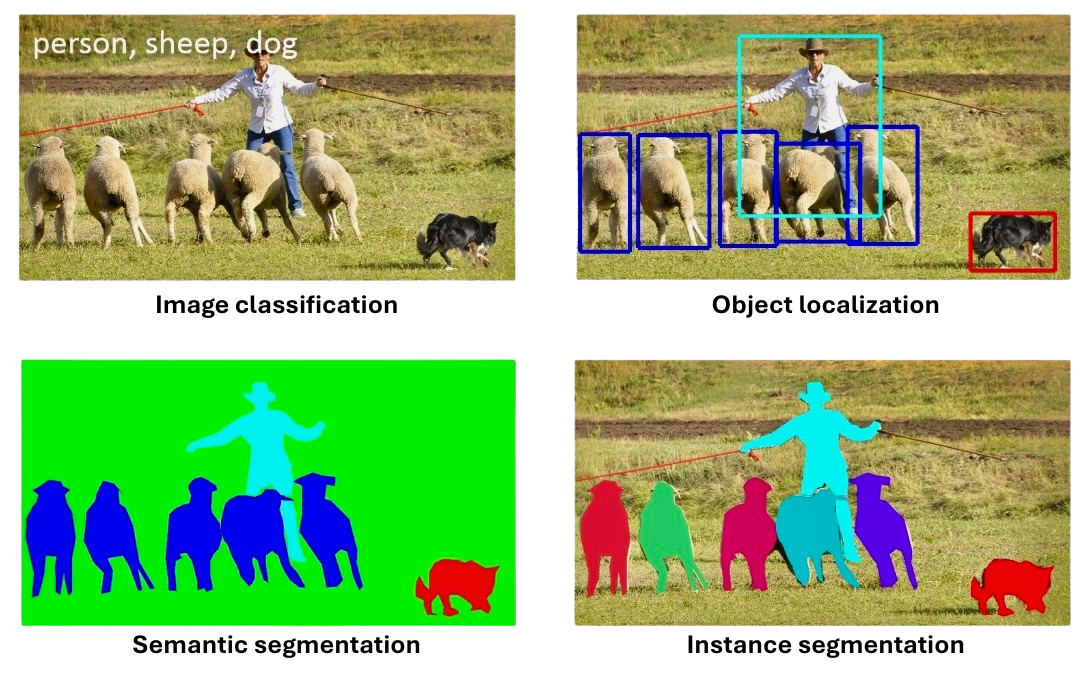
\includegraphics[width=0.75\linewidth]{imgs/Instance segmentation.png}
    \caption{Sample annotated image from the COCO \cite{lin2015microsoftcococommonobjects} dataset with a comparison of common computer vision tasks.}
    \label{fig:semantic}
\end{figure}

In this work, we focus exclusively on \textbf{instance segmentation}, as our goal is to estimate the number of neoplastic nuclei in histopathology images. This requires not only identifying which pixels belong to nuclei, but also distinguishing between adjacent ones. To this end, the output of our models consists of binary masks where each predicted nucleus after postprocessing will be labeled as a separate instance. This approach allows us to precisely count, localize, and analyze individual nuclei, which would not be possible with standard semantic segmentation.
\section{Convolutional Neural Networks (CNNs)}
This section introduce Convolutional Neural Networks (CNNs) in the context of instance segmentation. We begin with a general overview of CNNs and their key components. Then, we discuss how CNNs are used as encoders to extract features from input images, and how these features are processed by segmentation architectures to produce pixel-wise predictions.
\subsection{Overview}
A Convolutional Neural Network (CNN) is specialized type of artificial neural network designed to process data with a grid-like structure, such as images. through convolutional layers that capture sparial hierarchies within data. CNNs have demostrated superior performance in numerous visual recognition tasks including image classification, object detection, and instance segmentation.\\
A typical CNN architecture consists of the following core components:
\begin{itemize}
    \item \textbf{Convolutional layers}: these layers perform convolution operations using a set of learnable filters (kernels). Given an input tensor $\mathbf{X}\in\mathbb{R}^{H\times W\times C}$, where $H$, $W$, and $C$ represent the height, width, and number of input channels, the convolution with filter $\mathbf{K}_i\in \mathbb{R}^{k\times k\times C}$ produces and output feature map $\mathbf{Y}_i\in \mathbb{R}^{H\times W}:$
    \begin{equation}
        \mathbf{Y}_i=\mathbf{X}*\mathbf{K}_i+b_i
    \end{equation}
    where $*$ denotes the discrete convolution operator, and $b_i\in\mathbb{R}$ is a learnable bias term. The convolution operation can highlight specific patterns such as edges, textures, or more complex shapes.
    \item \textbf{Activation functions}: After convolution, an activation function is applied to introduce non-linearity into the network. Common activation functions include Rectified Linea Unit (ReLU), sigmoid. and hyperbolic tanget (tanh). ReLU, defined as $f(x)=max(0,x)$, is particularly popular due to its simplicity and ability to mitigate the vanishing gradient problem.
    \item \textbf{Pooling layers}: pooling operations reduce the spatial dimensions of feature maps. Max pooling, retaining the maximum value within a local region $\mathcal{R}\subset \mathbb{R}^{p\times p}$, is frequently used:
    \begin{equation}
        Y_{i,j}=max_{(m,n)\in\mathcal{R}}X_{i+m,j+n}
    \end{equation}
    Pooling layers emphasize dominant features while discarding irrelevant details. Alternatively, average pooling, which computes the evarage, is also frequently used.
    \item \textbf{Fully connected layers}: typically placed at teh end of CNN architectures for classification or regression tasks, these layers integrate extracted features into high-level representations to generate final predictions.
\end{itemize}
CNNs leverage hierarchical feature extraction, capturing local features initially (e.g.,edges, corners) which progressively combine into more global, semantic features. This hierarchical structure  enables CNNs to efficiently learn invariance and robust visual representations.
\begin{figure}[h]
    \centering
    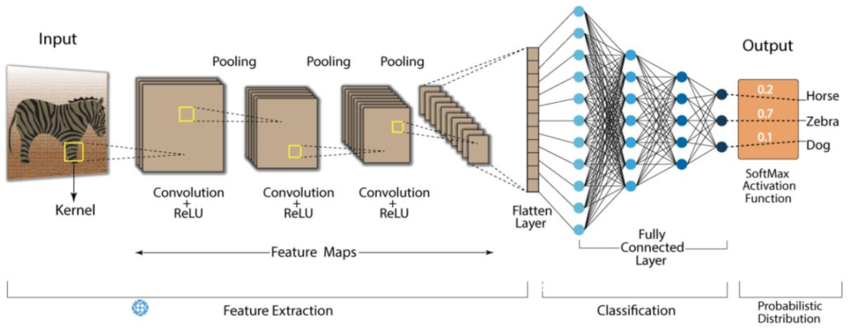
\includegraphics[width=0.8\textwidth]{imgs/CNN.png}
    \caption{Basic CNN architecture. Reproduce from researchgate.com}
\end{figure}
\subsection{Segmentation architecture}
A \textbf{segmentation architecture} is the component of semantic segmentation model that converts high-level feature maps from the encoder into pixel-wise class predictions. While the encoder focuses on extracting semantic information by downsampling the input,the segmentation architecture restores spatial resoltion to produce segmentation masks.\\
Typical segmentation architecture designs use a combination of upsampling layers, skip connections, and convolutions to progressively refine features and recover spatial details. The choice of the architecture affects both the accuracy and efficiency of the segmentation model. \\
For this work there are several widley used CNN-base segmentation architectures, including UNet, and UNet++. As described in chapter \ref{sec:model} we used a UNet with two heads.\\

\noindent\textbf{UNet}\\

\noindent UNet is a CNN architecture specifically designed for instance segmentation tasks, pariomedical image analysis. It was introduced in \cite{DBLP:journals/corr/RonnebergerFB15} to address the challenge of achieving precise pixel-level segmentation with limited data. 
\section{Distance maps}
\section{Watershed algorithm}
\chapter{Dataset}
\label{sec:dataset}
The analysis of nuclear features in histopathology images has long been recognized as a crucial aspect of cancer research and diagnosis. The part that seems like a bottleneck is the limited size of the most publicy available dataset for nuclei segmentation and classification, and often suffering from sparse labelling or sampling bias.\\
To address this limitations, Gamper et al. (2019) 
\cite{gamper2019pannuke,gamper2020pannuke} introduce and extended PanNuke, an open pan-cancer a semi-automatically obtained for nuclei instance segmentation and classification dataset.

%% Sezione
\section{Materials}
PanNuke is created through multiple model combinantions with already existing public data for nuclei classification$/$segmentation. To produce the proposed dataset have been sampled patches randomly extracted from a Whole Slide Image (WSI), using 19 different TCGA tissue types and other internal dataset for prostate, colon, ovarian, breast and oral tissue.\\
In total, 455 visual field were collected, of which 312 were randomly sampled from more than 200.000 H\&E-stained WSI, using a random approach to chose the patch allowed the authors to address the selection bias present in available public dataset. To overcome the scarity of ground truth and the unreliability of manual labeling, have been adopted a three stream approach regarding segmentation, classification and detection models.\\
For the segmentation stream, the authors used the Kumar \cite{article} dataset and CPM17 \cite{vu2018methodssegmentationclassificationdigital} dataset. For the detection stream, additional images were extracted from TCGA and the Bone Morrow \cite{10.1007/978-3-319-24574-4_33} dataset  . The classification stream, the nuclei were labeled using MonuSeg, ColonNuclei, SPIE cellularity challenge data, and the Nuclei Attribute dataset, ensuring a diverse set of nuclear categories.\\

\begin{table}[ht]
\centering
\caption{PanNuke Nuclei Categories from initial datasets. Reproduce from \cite{gamper2020pannuke}}
\label{tab:pannuke_init}
\resizebox{\textwidth}{!}{%
\begin{tabular}{lrrrrrrr}
\hline\hline
 & \multicolumn{7}{c}{\textbf{PanNuke Nuclei Categories}} \\
\cline{2-8}
\textbf{Dataset} & \textbf{Neoplastic} & \textbf{Non-Neo Epithelial} & \textbf{Inflammatory} & \textbf{Connective} & \textbf{Dead} & \textbf{Non-Nuclei} & \textbf{Total} \\
\hline
MoNuSeg          & 5,927 &   836 & 1,698 &   906 &   0 &   0 &   9,367 \\
Colon Nuclei     & 4,685 & 7,544 & 6,003 & 4,468 & 2,547 &   0 &  25,247 \\
BreastPathQ      & 9,802 &     0 & 2,139 &     0 &   0 &   0 &  11,941 \\
Nuclei Attribute &     0 &     0 &     0 &     0 &   0 & 500 &     500 \\
\hline
\textbf{Total}   &20,414 & 8,380 & 9,840 & 5,374 & 2,547 & 500 & 47,055 \\
\hline\hline
\end{tabular}%
}
\end{table}
\section{Method}
The authors followed three pathways to abtaind the validated dataset. These three pathways are segmentation, detection and classification. Using the CNN trained on patches extracted from the datasets in Table 1, they classified all the labeled nuclei part of the above datasets mentioned, which were then verified by a team of pathologists and classified by the PanNuke categories.\\
After, they took 2,000 patches from more than 20,000 WSI in 19 tissues obtained from a TCGA.
The models predictions were evaluated in terms of uncertainty, like a clear misclassification. The expert pathologists re-annotated these difficult cases, and the corrected annotations were used to retrain the models. 
\begin{figure}[h] % l'opzione [h] cerca di posizionare l'immagine "here"
    \centering
    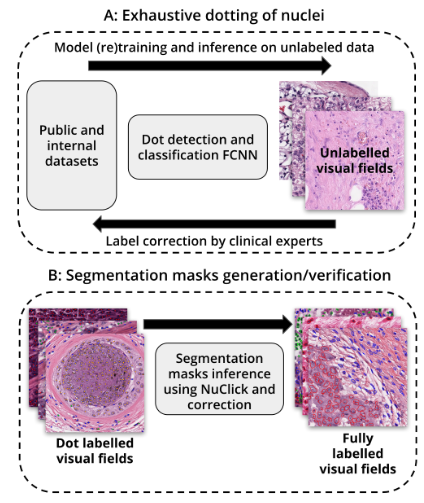
\includegraphics[width=0.45\textwidth]{imgs/pannuke_annotations.png}
    \caption{Illustration of PanNuke for label and verificationthe. Reproduce from \cite{gamper2020pannuke}}
    \label{fig:esempio}
\end{figure}
Then proceed to Part A of annotation process Figure 1.1. After a total of 7 iterations of the process, pathologists would evaluate and re-label the detected and classified nuclei.\\
To generate the segmentation masks they use NuClick \cite{jahanifar2019nuclick}, that brings an accurate segmentation mask from a single point. 
\section{Class Distribution}
\label{sec:classdistribution}
In evarage, most nuclei types that have been provided belongs in all tissues considered in PanNuke.
\begin{figure}[h]
  \centering
  \begin{minipage}{0.45\textwidth}
    \centering
    \includegraphics[width=\linewidth]{imgs/class_distributionù.png}
    \caption{Class distribution. Reproduce from \cite{gamper2020pannuke}}
  \end{minipage}\hspace{2cm}
  \begin{minipage}{0.3\textwidth}
    \centering
    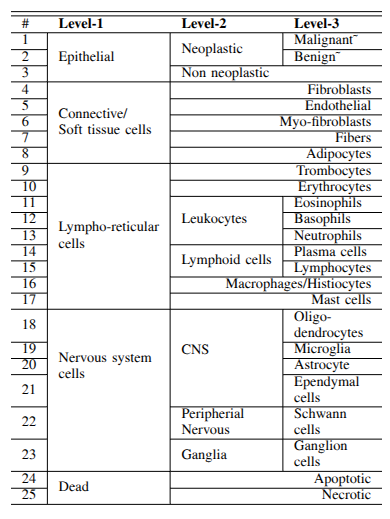
\includegraphics[width=\linewidth]{imgs/class_tab.png}
    \caption{Nuclei categories. Reproduce from \cite{gamper2020pannuke}}
  \end{minipage}
\end{figure}
PanNuke defines nuclei into five categories, tab 1.3: \textbf{Neoplastic} includes any type of tumor, malignant or benign, therefore includes carcinomas, sarcomas, melanomas, lymphomas, etc. Those tumors are originate from different cell types: carcnimoas from epithelial; sarcomas from lymphoid cells etc.\\
\textbf{Non-neoplastic} covers everything else, thus different categories from normal to inflammatory, metaplastic, degenerative, etc.\\
\textbf{Connective} cells have the potential to become tumors.\\
\textbf{Inflammatory} cells include macrophage and lymphoid, unlike connective cells, inflammatory cells cannot become plastic.\\
\textbf{Dead cells} can arise from neoplastic or non-neoplastic.\\

In figure 1.2 we can observe that the distribution of the total nuclei count per tissue and per class changes between tissue types. We observe that there is a strong imbalance reflects the biological prevalence of cell types in histopathology slides that will become a challenge for deep learning models. In particular, the nucleis categoriesed dead are rare, therefore will be difficult to segment and classify.\\
Overall, the class distribution prove that PanNuke offers both large quantities of common cell types and valuable examples of underrepresented nuclei, reaching a realistic dataset that mirrors the cases that could present in clinical practice.

\section{Dataset Statistics}
The PanNuke dataset provides nuclei annotations across 19 tissue types, with each nucleus labeled according to one of five clinically relevant categories. The dataset contains 189,744 nulei annotated at the instance level.\\
For the purpose of this work, only neoplastic nuclei where considered. This choice was motivated by the specific objective of our study, which focused on identifying and counting malignant cells. In practice, the ground truth masks were converted in bianry masks, where each positive pixel belong to a neoplastic nucleo and the remaining pixels were just merged with the background.\\

By restricting the dataset to neoplstic nuclei, the resulting distribution is imbalanced compared to the full PanNuke schema.

\chapter{Methodology}
\label{sec:methodology}
The workflow of the proposed project is a standard deep learning pipeline for nuclei segmentation with differential tuning for detecting and counting the neoplastic nuclei in histopathology images.

In the first place, the raw images and object annotations are pre-processed to produce the model inputs. More specifically, original instance masks in PanNuke are converted into binary masks indicating the presence of neoplastic nuclei, and distance maps are calculated to encode the spatial interaction between neighbouring nuclei.

The heart of the system is a U-Net \cite{DBLP:journals/corr/RonnebergerFB15} network with an additional two output heads. This multi-head design can make the model learn pixel-wise classification and spatial structural information simultaneously, which is beneficial to generalization and robustness, and can also enhance the performance of nuclei segmentation and counting task.

\subsection{Tool and environment} The realization of the project that involves the training of models and the execution of the pipeline demanded for tools. The complete project is written in Python 3.12. \

\noindent\textbf{Hardware environment}\

\noindent The complete pipeline was run on a workstation having the following hardware components: \begin{itemize} 
    \item \textbf{CPU}: AMD Ryzen 5 9600X, 6C/12T 
    \item \textbf{GPU}: NVIDIA RTX 3080 Ti 11 GB
    \item \textbf{RAM}: 32 GB DDR5, 6000 MHz 
    \item \textbf{OS}: Linux (Ubuntu) 64 bit 
    \item \textbf{CPU Cache}: L3 38 MB 
\end{itemize} 
This setting was computationally feasible for our model training.

\subsection{Pipeline} The pipeline was constructed to guarantee that the entire workflow, from data pre-processing up to the automated model evaluation, was reproducible: from the preparation of the data to the automatic evaluation of the models. The entire set of procedure is coordinated by the main script \texttt{main.py}. The overall framework for automatic nuclear instance segmentation can be observed in Fig. 1 and the proposed network in Fig. 2

\section{Problem statement} The aim of this study is to develop and investigate a segmentation framework specifically designed for the detection and counting of \textbf{neoplastic nuclei} from histopathology images. PanNuke annotates some other forms of nuclei in addition to other surrounding entities (multi-class) whereas ours is exclusive to cancerous nuclei (multi-nominal) translating the original multi-class problem to a binary segmentation problem.

Another objective is to study the differences in performances and counting precision when different image representations (i.e., RGB, hematoxylin-extracted H\&E channels, blue colormaps, grayscale) are used. In this frame, the main points of research can be listed as: \begin{itemize} \item Binary masks and distance maps learned from PanNuke instance annotations serve as trustworthy supervisory signals for both segmentation and nuclei separation? \item What is the effect of the input modality on the model's capability to segment and count mitotic nuclei? \end{itemize}

Addressing these questions are key to the strength of the proposed pipeline, and its potential for deployment in real-life digital pathology scenarios.

\section{Pre processing}
Preprocessing is a fundamental step, as it adapts the raw PanNuke data to the specific objective of segmenting and counting neoplastic nuclei. Since, the main goal is segment and count the neoplastic nuclei, this requires transforming the instance-level annotations into binary masks, as well as generating distance maps that help to separete the different cluster of nucleis.\\
In addition, the original RGB images were processed using blu colormaps, hematoxylin-extracted H\&E channels and grayscale, to understand how various input affect segmentation performance.
\subsection{Dataset files}
\label{sec:datafiles}
The raw PanNuke dataset is organized into three folder inside each folder there are 3 files .npy:

\begin{enumerate}
    \item \textbf{types.npy}: contains the categorical label of each nucleus. Since this project does not address nuclear classification, this file is not used.
    
    \item \textbf{mask.npy}: contains $N$ images, each with a size of $256 \times 256$ pixels and 6 channels.  
    The first five channels correspond to the instance maps of the nuclear categories described in Section~\ref{sec:classdistribution}.  
    Specifically, the first channel encodes the instance map of neoplastic nuclei in the $n$-th image, the second channel the instance map of non-neoplastic epithelial nuclei, and so on.  
    The sixth channel is a binary mask that includes all nuclei, regardless of category, in the $n$-th image.
    
    \item \textbf{image.npy}: contains $N$ images, each with a size of $256 \times 256$ pixels and 3 channels, representing the original RGB images.
\end{enumerate}
\begin{center}
    \begin{tikzpicture}
        \node (img1) {\includegraphics[height=3cm]{imgs/class_distributionù.png}};

        \node (img2) at (img1.south east){\includegraphics[height=3cm]{imgs/class_distributionù.png}};
    \end{tikzpicture}
\end{center}
\subsection{Image Preprocessing}
The image preprocessing was developed to evaluate the impact of different input on the main task. 
The raw dataset provides RGB images described in Section~\ref{sec:datafiles}. 
From these images, additional channels were derived to highlight nuclear structures and assess whether color information affects models performances. 

Specifically, four different input variants were considered:

\begin{itemize}
    \item \textbf{RGB}: the original $256 \times 256$ image RGB.
    \item \textbf{Hematoxylin (H\&E)}: images obtained by color deconvolution, where the hematoxylin channel is extracted to emphasize nuclear morphology \cite{ruifrok2001quantification}.
    \item \textbf{Blue colormap}: a transformed representation where intensity values are mapped to a blue color scale, enhancing contrast between nuclei and background.
    \item \textbf{Grayscale}: single-channel images representing intensity only, without color information.
\end{itemize}
By preprocessing the dataset into these four modalities, the experimental pipeline allows a direct comparison of how different color representations influence segmentation accuracy. 
\begin{figure}[h!]
    \centering
    % Riga 1
    \begin{subfigure}{0.45\textwidth}
        \centering
        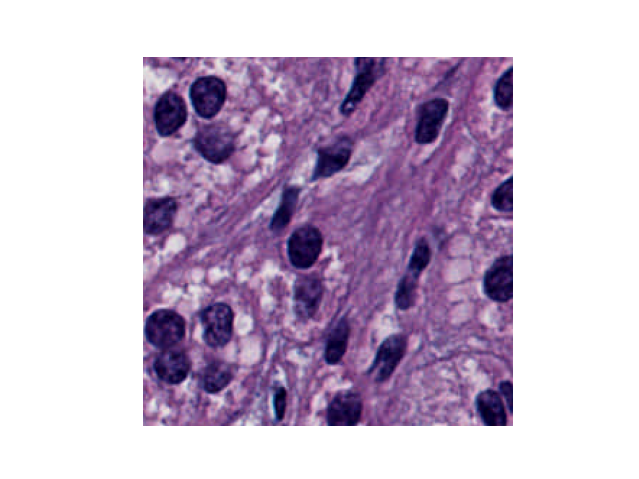
\includegraphics[width=\linewidth]{imgs/RGB.png}
        \caption{RGB}
    \end{subfigure}
    \hspace{0.2cm}
    \begin{subfigure}{0.45\textwidth}
        \centering
        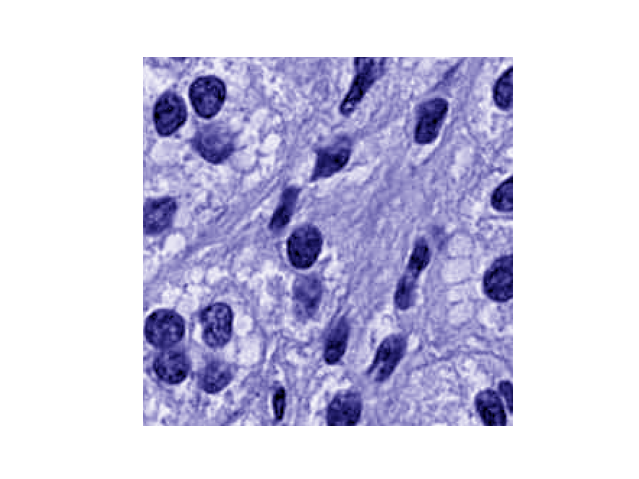
\includegraphics[width=\linewidth]{imgs/HE.png}
        \caption{Hematoxylin}
    \end{subfigure}
    
    \vspace{0.4cm} % spazio verticale fra le righe
    
    % Riga 2
    \begin{subfigure}{0.45\textwidth}
        \centering
        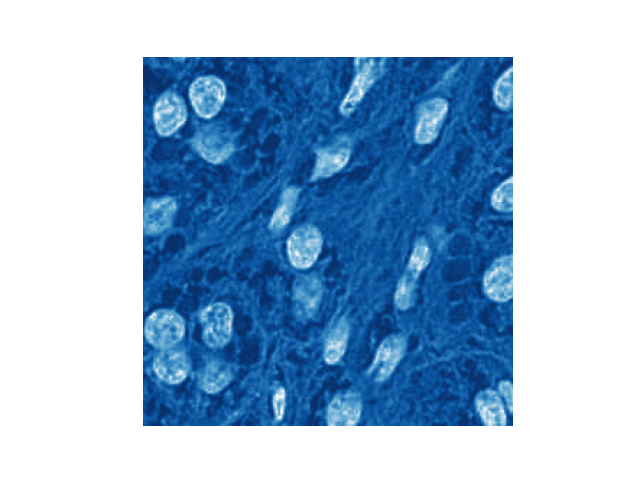
\includegraphics[width=\linewidth]{imgs/Blu.png}
        \caption{Blu channel}
    \end{subfigure}
    \hspace{0.2cm}
    \begin{subfigure}{0.45\textwidth}
        \centering
        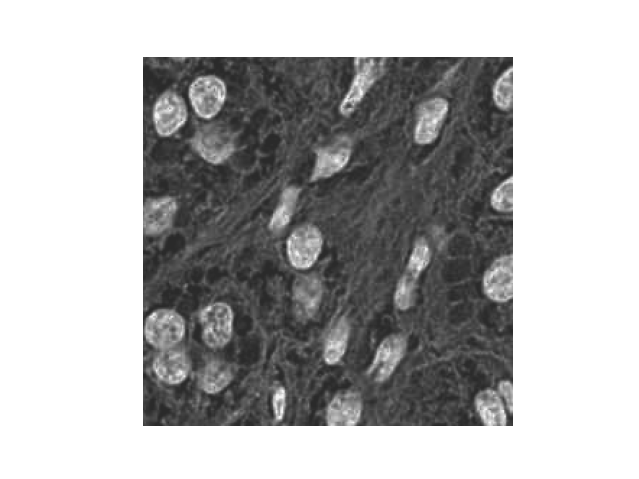
\includegraphics[width=\linewidth]{imgs/Gray.png}
        \caption{Gray scale}
    \end{subfigure}
    
    \caption{Each type of color representations used}
    \label{fig:quattro_immagini}
\end{figure}

\subsection{Mask Generation}
In the PanNuke datasets there are different files described in Section~\ref{sec:datafiles}, for this work will be use only a part of them. The task is to study the segmentation and counting of neoplastic cells. Therefore, the generation of binary masks and distance maps pivot on that goal.\\

\noindent\textbf{Binary masks}\\
\label{sec:maskgeneration}
From the file \texttt{masks.npy}, have been extracted the channel corresponding to the neoplastic cells. The image extracted is $256 \times 256$ and provide as an instance map, where every individual cell is assigned a unique label (e.g., 1, 2, 3,\dots). Subsequently, to obtain a binary mask, all non-zero pixel in the instance map are mapped to 1, while background pixels remain 0. The instance map $I$, the corresponding binary mask $B$:
\begin{center}
$
B(i) = 
\begin{cases}
1 & \text{if } I(i) > 0 \\
0 & \text{if } I(i) = 0
\end{cases}
$
\end{center}
where $i$ denote a pixel location. Before being used each binary mask is converted into a three-channel trugh the function \texttt{\_mask\_to\_3ch}:
\begin{itemize}
    \item \textbf{Body}: Each positive pixel is assigned to a nucleus.
    \item \textbf{Background}: Each positive pixel not belonging to any nucleus, therefore is part of the background.
    \item \textbf{Border}: a contour around each nucleus, obtained by applying a morphological erosion to the binary mask and the substracting the eroded mask from the original.
\end{itemize}
This three-channel encoding brings to distinguish nuclear region from background, therefore increase the segmentation performance.\\
\begin{figure}[H] % l'opzione [h] cerca di posizionare l'immagine "here"
    \centering
    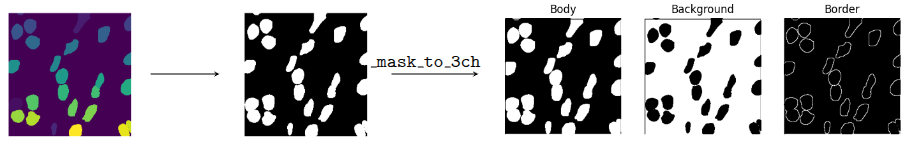
\includegraphics[width=1\textwidth]{imgs/binarymask_transform.png}
    \caption{Overview of the proposed approach for the transformation from instance map to binary mask with 3 channels}
    \label{fig:esempio}
\end{figure}
\noindent\textbf{Distance maps}\\
Beside the binary masks, the pre-processing pipeline also produce distance maps (265765) that give pixel-wise geometric information on nuclear shape. For H\&E images, every distance map consists of two channels representing the horizontal (H) and vertical (V) distance of the pixels to the centroid of their nuclei. This representation, spurred by HoVer-Net \cite{graham2019hovernet}, enables the model to disentangle touching or overlapping nuclei by learning their spatial configuration.

Generation process will begin from the neoplastic nuclei instance maps obtained from \texttt{mask.npy}. The result is a standarised instance map, in which each nucleus has been labelled by an unique index. The class \texttt{GenInstanceHV}, next, computes the horizontal and vertical distances for all pixels within the nucleus, normalizing them between $-1$ and $1$. The pipeline also involves post-processing to account for duplicated labels due to data augmentation, and filtering very small objects.

The resulting ground truth is a 2-array: binary mask containing neoplastic nuclei, and a pair of distance maps H and V. These will be used later as supervision targets for a segmentation head and a regression head of the U-Net: the segmentation head outputs imposingly binary masks, the regression head predicts dense HV maps.

This formulation helps the model to learn the categorical and structural information jointly, which further enhances the stability of nuclei segmentation and counting.
\begin{figure}[htbp] % o [H] con \usepackage{float}
\centering
\begin{tikzpicture}[node distance=8cm, >=stealth]
  % immagini
  \node (img1) {
\includegraphics[width=0.30\textwidth]{imgs/instance.png}};
  \node (img2) [right of=img1, xshift=1cm]
        {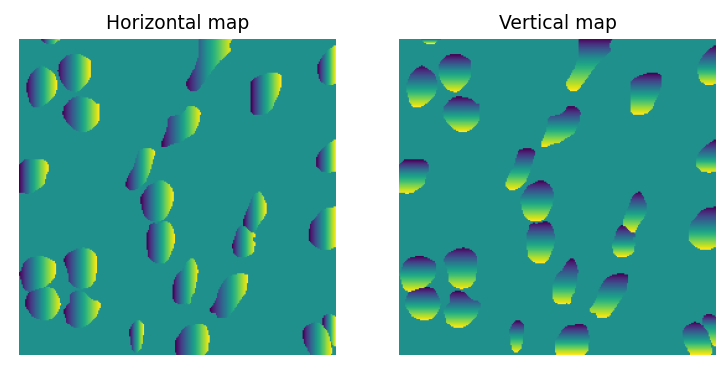
\includegraphics[width=0.40\textwidth]{imgs/Distancemaps.png}};

  % freccia con etichetta sopra
  \draw[->] (img1.east) -- (img2.west)
    node[midway, above]{\texttt{GenInstanceHV}};
\end{tikzpicture}
\caption{Overview of the proposed approach for the generation of distance maps}
\label{fig:esempio}
\end{figure}
\subsection{Data Augmentation}
To increase variability and reduce the risk of overfitting, the dataset was augmented during training using simple but effective geometric transformations. 
All augmentation was implemented directly in the custom \texttt{DataGenerator} class, which inherits from \texttt{keras.utils.Sequence} and dynamically loads and transforms data on the fly. 

The applied transformations were:
\begin{itemize}
    \item \textbf{Horizontal and vertical flipping}: images and their corresponding masks were randomly flipped along the horizontal or vertical axis with probability 0.5.
    \item \textbf{Random rotations}: patches were rotated by multiples of 90 degrees, ensuring consistent orientation between the image, binary mask, and distance maps.
\end{itemize}

These transformations preserve the semantic structure of nuclei while increasing diversity in the training set. 
By applying them stochastically at each epoch, the effective dataset size is multiplied, leading to improved generalization of the model. 
It is important to note that both the segmentation masks and the distance maps were augmented consistently with the corresponding images to maintain spatial alignment. 

In addition to geometric transformations, the \texttt{DataGenerator} also supports different input representations (RGB, hematoxylin channel, blue colormap, and grayscale), enabling a systematic comparison of model performance across varying image modalities. All transformations were applied only to the \textbf{train} subset, while \textbf{val} and \textbf{test} remained in their original form.\\

Before each augmentation session, the script sets a global seed that synchronizes the random number generators of \textbf{NumPy} and \textbf{cv2} (OpenCV). This ensures that the same batch of images can always be reproduced and anomalies can be consistently identified.
\section{Model Architecture}
\label{sec:model}
The proposed network is inspired by the U-Net architecture \cite{DBLP:journals/corr/RonnebergerFB15}, a widely used encoder–decoder structure for biomedical image segmentation. 
U-Net consists of a contracting path, which progressively captures semantic context through convolutional and downsampling operations, and an expansive path, which combines this context with high-resolution spatial information via skip connections. 
This design enables precise delineation of cellular structures even when only limited training data is available.

In our implementation, the encoder is composed of successive convolutional blocks with batch normalization, ReLU activation, and dropout for regularization. 
The number of filters doubles at each downsampling step (32, 64, 128, 256, 512), while max pooling layers reduce the spatial resolution by a factor of two. 
The bottleneck layer captures high-level semantic features with 512 filters before entering the decoder.

The decoder mirrors the encoder with upsampling layers, concatenations with the corresponding encoder features, and convolutional refinements. 
This symmetric structure ensures that contextual information extracted at low resolutions is effectively fused with fine-grained spatial details.

\noindent\textbf{Multi-head design.}  
To better address the task of nuclei segmentation and separation, the model has been extended with two task-specific output heads, inspired by the HoVer-Net approach \cite{graham2019hovernet}:  
\begin{itemize}
    \item \textbf{Segmentation head (seg\_head)}: a 1$\times$1 convolution followed by a softmax activation outputs a 3-channel probability map corresponding to \textit{body}, \textit{background}, and \textit{border}. This representation explicitly encodes both nuclear regions and contours, which facilitates the separation of touching nuclei.  
    \item \textbf{Distance head (hv\_head)}: a parallel 1$\times$1 convolution followed by a linear activation outputs two channels encoding the horizontal (H) and vertical (V) distances of each pixel to the nucleus centroid. These distance maps provide strong geometric cues to further separate overlapping nuclei.  
\end{itemize}

\noindent\textbf{Advantages.}  
By combining semantic segmentation (seg\_head) with geometric regression (hv\_head), the network simultaneously learns categorical and structural information. 
This multi-task formulation improves robustness in crowded regions and enhances nuclei counting, while preserving the efficiency of an end-to-end trainable model.
\begin{figure}[H] % l'opzione [h] cerca di posizionare l'immagine "here"
    \centering
    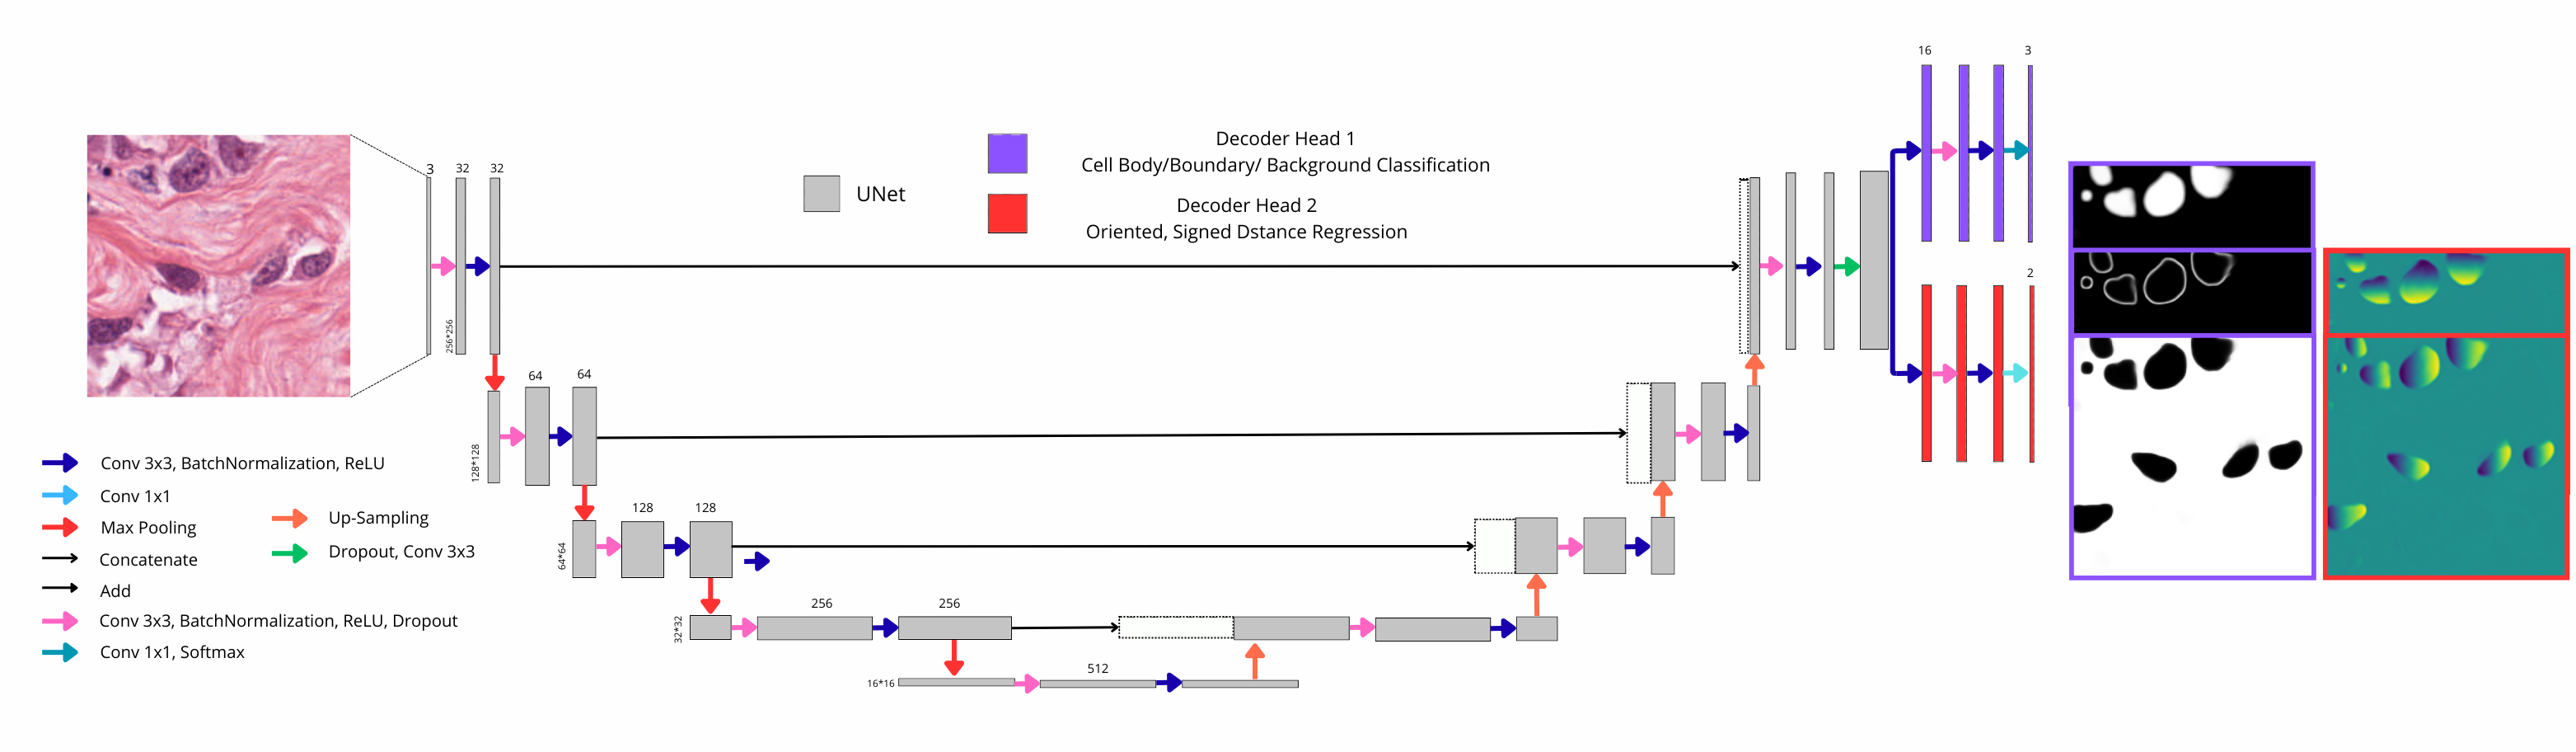
\includegraphics[width=1\textwidth]{imgs/model.png}
    \caption{Model architecture used}
    \label{fig:Unet}
\end{figure}
\section{Loss Function}
The model describred in Section~\ref{sec:model} is trained using a composite loss functino $\mathcal{L}^p+\mathcal{L}^d$ wich combines terms for pixel classificatino into $body$, $background$, $border$ ($\mathcal{L}^p$) and distance map regression in ($\mathcal{L}^d$).
In the following, we refer at each pixel $i$ and to the heads'output tensor as $\widehat{\mathbf{Y}}^p=[\widehat{\mathbf{Y}}^p_{ik}]\in [0,1]^{H\times W\times P}$, $\widehat{\mathbf{Y}}^d=[\widehat{\mathbf{Y}}^d_{ik}]\in \mathbb{R}^{H\times W\times R}$, respectively, where $P = 3$, $R = 2$, are the number of pixels classes and the number of distance maps, $N$ and $W$ mathes the height and width of the images in input. The ground truths (GT) are represented as $\mathbf{Y}^p$ and $\mathbf{Y}^d$.

A fundamental aspect to keep in mind when training a neural network models lies in the coice of an appropriate loss function. The loss function directly defines the model's optimization objective and this significantly influences ints performance and ability to handle common challenges such as class imbalance and structural detail preservation.

As described before the U-net proposed has 2 dirrent sets of weights: $w_0, w_1$ which refer to the weights $\mathcal{L}^p$ (hv\_head) and $\mathcal{L}^d$ (seg\_head). These 2 sets of weights are optimised jointly using the loss $\mathcal{L}$ defined as:

\begin{equation}
\mathcal{L} =
\underbrace{\lambda_a \mathcal{L}_a + \lambda_b \mathcal{L}_b}_{\text{hv\_head}} +
\underbrace{\lambda_c \mathcal{L}_c + \lambda_d \mathcal{L}_d}_{\text{seg\_head}}
\end{equation}
where $\mathcal{L}_a$ and $\mathcal{L}_b$ represent the regression loss for the distance maps predicted, $\mathcal{L}_c$ and $\mathcal{L}_d$ represent the loss with respect ot the output at the seg\_head, therefore the binary masks. $\lambda_a\dots\lambda_d$ are scalars that gives weight to the the loss. More precisly, we set $\lambda_b$ to 2 and the others scalars set to 1. \\

In practice, each component of the total loss corresponds to a specific learning objective. 
For the \textbf{hv\_head}, which predicts the horizontal and vertical distance maps, two terms are considered: 

\begin{itemize}
    \item \textbf{Mean Squared Error (MSE)}:  
    \begin{equation}
        \mathcal{L}_a = \frac{1}{N} \sum_{i=1}^{N} \| \mathbf{Y}^d_{i1} - \widehat{\mathbf{Y}}^d_{i1} \|^2 + \| \mathbf{Y}^d_{i2} - \widehat{\mathbf{Y}}^d_{i2} \|^2
    \end{equation}
    where $\mathbf{Y}^d_{i1}, \mathbf{Y}^d_{i2}$ denote the ground-truth horizontal and vertical distance maps at pixel $i$, and $\widehat{\mathbf{Y}}^d_{i1}, \widehat{\mathbf{Y}}^d_{i2}$ are the corresponding predictions. 
    This term enforces accurate regression of distance values. 
    
    \item \textbf{Gradient loss}:  
    \begin{equation}
        \mathcal{L}_b = \frac{1}{m} \sum_{i\in M} 
        \big( \| \nabla_x \mathbf{Y}^d_{i1} - \nabla_x \widehat{\mathbf{Y}}^d_{i1} \|^2 + \| \nabla_y \mathbf{Y}^d_{i2} - \nabla_y \widehat{\mathbf{Y}}^d_{i1} \|^2 \big)
    \end{equation}
    where $\nabla_x$ and $\nabla_y$ represents the Sobel gradient operator. in horizontal $x$ and vertical $y$ directions respectively. $m$ denotes total number of nuclear pixels within the image and $M$ denotes the set containing all nuclear pixels.
    This term enforces structural consistency and smoothness in the predicted distance maps, following the approach introduced by HoVer-Net \cite{graham2019hovernet}.
\end{itemize}

For the \textbf{seg\_head}, which outputs a 3-channel semantic segmentation mask (body, background, border), we employ two complementary terms: 

\begin{itemize}
    \item \textbf{Binary Cross Entropy (BCE)}:  
    \begin{equation}
        \mathcal{L}_c = - \frac{1}{N} \sum_{i=1}^{N} \sum_{k=1}^{P}\Big[ \mathbf{Y}^p_{ik}\log(\widehat{\mathbf{Y}}^p_{ik}) + (1 - \mathbf{Y}^p_{ik}) \log(1 - \widehat{\mathbf{Y}}^p_{ik}) \Big]
    \end{equation}
    where $\mathbf{Y}^p_{ik} \in \{0,1\}$ is the ground-truth label at pixel $i$ and $\widehat{\mathbf{Y}}^p_{ik} \in [0,1]$ is the predicted probability. 
    This loss penalizes incorrect pixel-wise predictions and is particularly effective under class imbalance. 
    
    \item \textbf{Dice loss}:  
    \begin{equation}
        \mathcal{L}_d = 1 - \frac{2 \sum_{i=1}^{N} \sum_{k=1}^{P} \mathbf{Y}^p_{ik} \widehat{\mathbf{Y}}^p_{ik} + \epsilon}{\sum_{i=1}^{N} \sum_{k=1}^{P} \mathbf{Y}^p_{ik} + \sum_{i=1}^{N} \sum_{k=1}^{P} \widehat{\mathbf{Y}}^p_{ik} + \epsilon}
    \end{equation}
    where $\epsilon$ is a smoothing constant to avoid division by zero. 
    This loss directly maximizes the overlap between predicted and ground-truth nuclear regions, mitigating the effect of class imbalance.
\end{itemize}

\section{Training Strategy}
The handle of train session is gave to \texttt{main.py}, that check and evaluate every sperimental sesio. 
\label{sec:train-strategy}

\subsection{Optimizer}
We train the network with the Adam optimizer \cite{kingma2014adam} using an initial learning rate $\eta_0=10^{-3}$ and
decoupled weight decay (AdamW-style) with coefficient $\lambda_{\mathrm{wd}}=10^{-4}$ \cite{loshchilov2019adamw}, leading to improved generalization compared to standard Adam, especially in vision tasks.\\
We adopt the standard $\beta_1{=}0.9$, $\beta_2{=}0.999$, and $\epsilon{=}10^{-8}$. In our experiments, the inclusion of a small decoupled weight decay yielded more stable training on this relatively small dataset.

\subsection{Learning rate scheduler}
THe learning rate is one of the most critical hyperparameters to set when training a model, directly affecting convergence speed, trainign stability, and overall model performance.\\
We employ \texttt{ReduceLROnPlateau} on the validation objective (monitoring \texttt{val\_loss}) with
reduction factor $\gamma{=}0.5$, patience of 3 epochs, and floor $\eta_{\min}{=}10^{-4}$.
Formally, letting $s_t$ be the best validation score up to epoch $t$ and $p$ the patience,
\[
\eta_{t+1} =
\begin{cases}
\max\{\gamma\,\eta_t,\ \eta_{\min}\} &\text{if } \forall\,\tau\in\{t-p+1,\ldots,t\}:\ s_\tau \text{ did not improve},\\[2pt]
\eta_t &\text{otherwise.}
\end{cases}
\]
This adaptive schedule reduces the step size only when progress stalls, avoiding abrupt changes typical of step schedules and promoting smoother convergence.

\paragraph{Early stopping and checkpointing.}
We adopt early stopping (patience $=5$, monitor \texttt{val\_loss}, with weight restoration of the best epoch) and model checkpointing (\texttt{save\_best\_only=true}). Together with the scheduler, these callbacks limit overfitting and select the best performing model without manual intervention.

\paragraph{Batching and generators.}
Mini-batches are produced on the fly by a custom \texttt{DataGenerator} (\S\ref{sec:datafiles}), which performs geometric augmentation on the training split (random flips and rotations by $k\cdot 90^\circ$) and keeps validation/test untouched. Targets are generated consistently for both heads: the 3-channel segmentation target (\emph{body}, \emph{background}, \emph{border}) for \texttt{seg\_head} and the two HV maps (plus focus mask) for \texttt{hv\_head}.

\paragraph{Reproducibility.}
We fix global seeds for NumPy and PyTorch (\texttt{SEED=42}) and enable deterministic behavior where possible; training runs on a single GPU (RTX~3080~Ti), with \texttt{keras} configured to use the \texttt{torch} backend.

\paragraph{Summary of hyperparameters.}
\begin{center}
\begin{tabular}{l l}
\hline
Optimizer & Adam ($\eta_0{=}10^{-3}$, $\beta_1{=}0.9$, $\beta_2{=}0.999$, decoupled WD $=10^{-4}$) \\
Scheduler & ReduceLROnPlateau (monitor=\texttt{val\_loss}, factor $=0.5$, patience $=3$, $\eta_{\min}{=}10^{-4}$) \\
Early stopping & patience $=5$, restore best weights \\
Checkpointing & best on \texttt{val\_loss} \\
Batch size & $8$ \\
Loss weights & $\text{seg\_head}:1.0$, $\text{hv\_head}:2.0$ \\
Epochs & $30$ (with early stop) \\
\hline
\end{tabular}
\end{center}
\section{Post-processing}
\label{sec:postprocessing}

The raw outputs of the multi-head U-Net model described in Sectio model, namely the probability maps from the \texttt{seg\_head} and the distance maps from the \texttt{hv\_head}, cannot be directly used for reliable nuclei counting. 
According to the notation in Section loss, this yield predictions $\widehat{\mathbf{Y}}^p$ and $\widehat{\mathbf{Y}}^d$ for the entire image, which are post-processed as illustrated in Fig1 and described below. 
This stage was partly inspired by the post-processing strategy proposed in HoVer-Net \cite{graham2019hovernet}, but adapted to the specific requirements of this work.

\subsection{Distance-based separation}
The distance maps predicted by the \texttt{hv\_head} are leveraged to separate adjacent or overlapping nuclei. 
For each pixel, the horizontal ($\widehat{\mathbf{Y}}^d_{i1}$) and vertical ($\widehat{\mathbf{Y}}^d_{i2}$) distance components are normalized into the range $[0,1]$ and each $\nabla_k,k=1,2$ rapresent the convolution with of a Sobel kernel:
\[
G_H = \nabla_1 \widehat{\mathbf{Y}}^d_{i1}, \qquad G_V = \nabla_2 \widehat{\mathbf{Y}}^d_{i2}.
\]
The combination of these gradients defines a boundary likelihood map:
\[
E = \mathbb{I}(max \big( 1 - \text{norm}(G_H), \, 1 - \text{norm}(G_V) \big)> \theta_1),
\]
which emphasizes nuclear contours and facilitates the detection of cell boundaries. The $\theta_1$ is binarizatino treshold, controls the amount of pixels considered as edges. The optimal value is set to $\theta_1=0.45$ for all models, it's been calculated on maximum of IoU see Section~\ref{sec:model}.
\subsection{Segmentation refinement}

The first step is to merge the predictions of the segmentation head. 
The model outputs three channels \emph{body}, \emph{background} and \emph{border} respectively $\widehat{\mathbf{Y}}^p_{i1}$, $\widehat{\mathbf{Y}}^p_{i2}$ and $\widehat{\mathbf{Y}}^p_{i3}$, which are combined into a binary probability map representing candidate nuclear regions :
\[
B = \mathbb{I}(\widehat{\mathbf{Y}}^p_{i1} + \widehat{\mathbf{Y}}^p_{i3} > \widehat{\mathbf{Y}}^p_{i2}),
\] 
This map highlights pixels likely to belong to nuclei and serves as a mask for subsequent refinement.

\subsection{Watershed instance segmentation}
Instance-level segmentation is obtained by applying a watershed algorithm to the boundary likelihood map. 
Candidate markers are generated by thresholding and morphological filtering, and the watershed is applied within the nuclear mask $B$. 
This yields a labeled instance map, where each connected component corresponds to a unique nucleus.\\
The topological surface used for the watershed transform is obtained from the complement of the predicted probability map, combined with the complement of the product between the binary nuclear mask and the inverse of the boundary map. 
This composite representation enhances the separation of touching nuclei and serves as the input for the watershed segmentation. 
The output is an instance segmentation map (or label map) $\hat{Y}_l$, in which each detected nucleus is assigned a unique positive integer label. 
Finally, objects with an area smaller than a threshold $\theta_2$, corresponding to the minimum acceptable nuclear size, are removed in order to discard spurious detections.

\subsection{Nuclei counting}
The final instance map is passed to a contour analysis stage that identifies individual nuclei and computes their bounding boxes. 
This step enables robust estimation of the nuclei count, which is then compared against the ground truth for evaluation.

\subsection{Overview}
The complete post-processing workflow can be summarized as follows:
\begin{enumerate}
    \item Merge segmentation outputs into a binary nuclear probability map.
    \item Normalize and process horizontal/vertical distance maps.
    \item Compute boundary likelihood using Sobel gradients.
    \item Apply watershed segmentation to obtain labeled instances.
    \item Remove small objects and artifacts.
    \item Count nuclei and extract contours for visualization.
\end{enumerate}
\begin{figure}[H] % l'opzione [h] cerca di posizionare l'immagine "here"
    \centering
    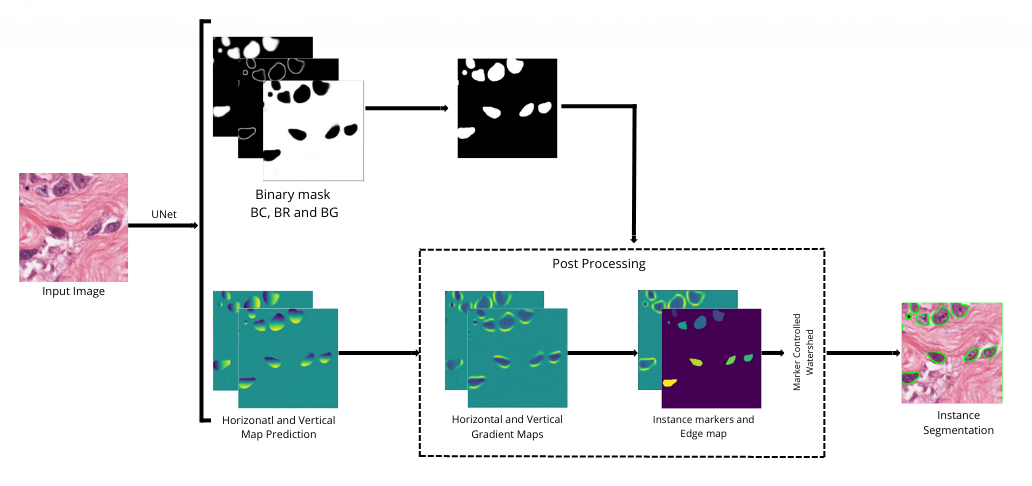
\includegraphics[width=1\textwidth]{imgs/overall.png}
    \caption{Model architecture used}
    \label{fig:postproc_overview}
\end{figure}
An overview of the full process --- from dataset to prediction, instance segmentation, and final counting --- is illustrated in Figure~\ref{fig:postproc_overview}.
\section{Evaluation Method}
In order to assess the performance of the model, we utilize both $quantitative$ and $qualitative$ evaluation methods.\\
The quantitative evaluation is based on objective numerical metrics calculated from a reserved test set. These metrics evaluate various facets of segmentation performance, offering a standardized means for comparing different types of colormaps applied to the input images.\\
Conversely, qualitative evaluation emphasizes the visual examination of high-resolution segmentation outputs. Additionally, due to the semi-automated nature of dataset annotations (as outlined in section~\ref{sec:dataset}), qualitative assessment also serves to highlight instances where model predictions may exceed ground truth accuracy.\\
The subsequent subsections elaborate on the metrics employed for quantitative assessment and the strategy used for qualitative analysis.\\
To gain deeper insights into the method, it is advantageous to decompose the problem into smaller sub-tasks and evaluate the method's performance on each one. Thus, for nuclear instance segmentation, we can categorize the problem into three distinct sub-tasks:
\begin{itemize}
    \item Distinguishing nuclei from the background
    \item Identifying individual nuclear instances
    \item Segmenting each identified instance
\end{itemize}
\subsection{Metrics}
\label{sec:metrics}
Two primary evaluation metrics have been utilized to gauge performance in nuclear instance segmentation:
\begin{enumerate}
    \item Ensemble Dice (DICE2) \cite{vu2019methods}
    \item Aggregated Jaccard Index (AJI) \cite{kumar2017dataset}
\end{enumerate}
Let X represent the ground truth and Y denote the predictions; specifically, X and Y refer to outcomes following post-processing. DICE2 calculates DICE for each nucleus using the Dice coefficient defined as follows:
\begin{equation}
    Dice = \frac{X\times(X\cap Y)}{(|X|+|Y|)}
\end{equation}
Meanwhile, AJI evaluates the ratio between aggregated intersection cardinality and aggregated union cardinality for sets X and Y.\\
These two evaluation metrics can only give a global perspective of the quality of the instance segmentation and do not help understanding of the performance on underlying sub-tasks.
Both DICE2, and AJI suffer a known limitation regarding the treatment of overlapping regions.
There is also a large negative effect on the score even for small gaps between two predictions, because predicted instances can overlap not only with the corresponding ground-truth but also with the neighbouring ones.
In the DICE2 framework this leads to over-penalisation, as pixels belonging to the estimated nucleus are treated as errors for a number of ground truth instances.
The AJI measure which pairs predictions and ground truth instances by using the highest intersection over union, is not as sensitive to this, but still influenced in the case where neighboring instances are completely missed.
This phenomenon is even more observed in challenging datasets like the one considered, in which there are nuclei presenting weak staining or unusual cell types to recognize, resulting in a larger proportion of nuclei that were not detected.
Due to the limitations of DICE2 and AJI, it is clear that there is a need for an improved reliable quantitaive measurement.\\

\textbf{Panoptic Quality}: We need to use another metric for accurate qantification and interpretability. Inspired by Hover-Net and originally proposed by \cite{kirillov2019panoptic}, panoptic quality (PQ) for nuclear instance segmentation is defined as:
\begin{equation}
\mathcal{PQ} =
\underbrace{\frac{|TP|}
{|TP| + \tfrac{1}{2}|FP| + \tfrac{1}{2}|FN|}}_{\text{Detection Quality (DQ)}}
\times
\underbrace{\frac{\sum_{(x,y) \in TP} IoU(x,y)}
{|TP|}}_{\text{Segmentation Quality (SQ)}}
\end{equation}
where $x$ denotes a Gt segment, $y$ y denotes a prediction segment and IoU denotes intersection over union. Each $(x,y)$ pair is mathematically proven to be unique over the entire set of prediction and GT segments if their IoU$(x,y)>0.5$. \\
Now, PQ can be read as follows: the $detection\ quality$ (DQ) is the $F_1$ Score, while $segmentation\ quality$ (SQ) can be interpreted as how close each correctly detected instance is to their matched GT.\\

To understand the correctly association with the sub-task claimed above, we use the following three metrics:
\begin{enumerate}
    \item DICE to measure the separation of all nuclei from the back-ground.
    \item Panoptic Quality as a unified score for camparison
    \item AJI
\end{enumerate}
\chapter{Results}
\label{chap:results}

This chapter presents the expertimental results obtained by training and evaluating, the proposed multi-head U-net model on the PanNuke dataset described in chapter \ref{sec:dataset}, using the methodology detailed in chapter \ref{sec:methodology}.\\
We begin by outlining a set of preliminary experiments that assess the impact of different input modalities (RGB, Hematoxylin, Blu colormap, Grayscale) to compare models performances, reporting quantitative results using standard segmentation metrics as described in Section~\ref{sec:metrics}, then analyse the nuclei counting accuracy, and complementing them with qualitative analysis of segmentation outputs on full images.\\
Unless otherwise stated, post-processing thresholds were set as in Section~\ref{sec:postprocessing}, with the foreground threshold $\theta_1$ tuned on validation by IoU on ground-truth labels and $\theta_2$ as the minimum instance area.

\section{Experimental setup}
All experiments were conducted under identical training conditions, as detailed in Chapter~\ref{chap:methodology}. 
Each model was trained for a maximum of 30 epochs with early stopping, using Adam optimizer with weight decay, ReduceLROnPlateau scheduler, and a batch size of 8. 
For each preprocessing modality (RGB, Hematoxylin, Blue, Gray), a separate model was trained and tested using the same split of training/validation data.

Performance evaluation was carried out using both segmentation metrics (Dice, IoU, AJI, PQ) and counting metrics (MAE, Pearson correlation $\rho$, coefficient of determination $R^2$). 
Post-processing was applied to all model predictions before metric computation to ensure consistency.

\section{Segmentation performance}

The final evaluation on the test set, as shown in tables~\ref{tab:iou-results} and ~\ref{tab:pix-binary}, the model with RGB images achieves the highest scores across all metrics.\\
Among the remaining input modalities, the Hematoxylin input performs moderately well,  
Table~\ref{tab:iou-results}  summarizes the instance-level performance using DICE2, AJI, PQ, SQ and DQ (Section~\ref{sec:metrics}). 
PQ is further factorized into detection quality (DQ) and segmentation quality (SQ), providing a more interpretable view on missed detections vs. mask quality.

\begin{table}[ht]
\centering
\caption{Instance-level segmentation performance across input modalities. Scores are averaged over the test set.}
\label{tab:iou-results}
\small
\begin{tabular}{lccccc}
\toprule
\textbf{Input} & \textbf{DICE2} $\uparrow$ & \textbf{AJI} $\uparrow$ & \textbf{DQ} $\uparrow$ & \textbf{SQ} & \textbf{PQ}\\
\midrule
RGB         & \textbf{0.601} & \textbf{0.527} & \textbf{0.640} & \textbf{0.701} & \textbf{0.477}\\
Hematoxylin & 0.593 & 0.514 & 0.635 & 0.689 & 0.468\\
Blue        & 0.556 & 0.450 & 0.585 & 0.670 & 0.387\\
Grayscale   & 0.586 & 0.501 & 0.625 & 0.692 & 0.444\\
\bottomrule
\end{tabular}
\end{table}

\noindent\textbf{Discussion.} 
Consistent with the literature on H\&E images, RGB and Hematoxylin inputs lead to higher PQ and AJI than Blue; Grayscale remains competitive, suggesting that much of the discriminative signal lies in structure rather than color. 
As discussed in Section~\ref{sec:metrics}, DICE2 and AJI tend to over-penalize overlaps in crowded regions; PQ mitigates this by decoupling detection and mask quality.\\

Besides instance metrics, we also report a pixel-wise IoU and F1 score on the binary foreground ($\text{body}\cup\text{border}$ vs background), as a sanity check for under/over-segmentation:

\begin{table}[ht]
\centering
\caption{Pixel-wise foreground segmentation (binary) on the test set.}
\label{tab:pix-binary}
\small
\begin{tabular}{lcc}
\toprule
\textbf{Input} & \textbf{IoU} $\uparrow$ & \textbf{F1} $\uparrow$ \\
\midrule
RGB         & \textbf{0.656} & \textbf{0.870} \\
Hematoxylin & 0.641 & 0.863 \\
Blue        & 0.582 & 0.834 \\
Grayscale   & 0.635 & 0.861 \\
\bottomrule
\end{tabular}
\end{table}

\section{Counting performance}
To evaluate the counting performance, we compare the number of predicted instances with the number of ground-truth instances, both obtained after post-processing. 
Let $\hat{n}_i$ and $n_i$ denote the predicted and ground-truth nuclei counts for image $i$, respectively, with $i=1,\dots,N$.

The following metrics are employed:

\begin{itemize}
    \item \textbf{Mean Absolute Error (MAE)}: measures the average absolute deviation between predicted and ground-truth counts,
    \begin{equation}
        \mathrm{MAE} = \frac{1}{N}\sum_{i=1}^{N} \left| \hat{n}_i - n_i \right|.
    \end{equation}

    \item \textbf{Pearson correlation coefficient} $\rho$: quantifies the degree of linear correlation between predictions and ground truth,
    \begin{equation}
        \rho = \frac{1}{N-1}\sum_{i=1}^N 
        \left(\frac{\hat{n}_i - \mu_{\hat{n}}}{\sigma_{\hat{n}}}\right)
        \left(\frac{n_i - \mu_{n}}{\sigma_{n}}\right),
    \end{equation}
    where $\mu_{\hat{n}}, \sigma_{\hat{n}}$ are the mean and standard deviation of the predicted counts, and $\mu_{n}, \sigma_{n}$ are the mean and standard deviation of the ground-truth counts.

    \item \textbf{Coefficient of determination} $R^2$: Cell counting performance represents the ability to determine cellular composistion \cite{kirillov2019panoptic}. It can be quantified via the $coefficient\ of\ determination$ $\textbf{R}^2$ to assess the correlation between the predicted and true counts as:
    \begin{equation}
        R^2 = 1 - \frac{\sum_{i=1}^N (n_i - \hat{n}_i)^2}{\sum_{i=1}^N (n_i - \mu_{n})^2},
    \end{equation}
    where the numerator corresponds to the residual sum of squares (RSS) and the denominator to the total sum of squares (TSS).
\end{itemize}

\subsection{Scatter plot analysis}
Counting performance was evaluated by comparing the number of predicted nuclei against ground truth counts after post-processing. 
Figure~\ref{fig:scatter_counts} shows the scatter plots for the four input modalities, with each point representing one test image. 
The dashed line denotes the ideal $y=x$ relationship. 
The closer the points lie to this line, the more accurate the model prediction.

\begin{figure}[ht]
\centering

\begin{minipage}{0.45\textwidth}
    \centering
    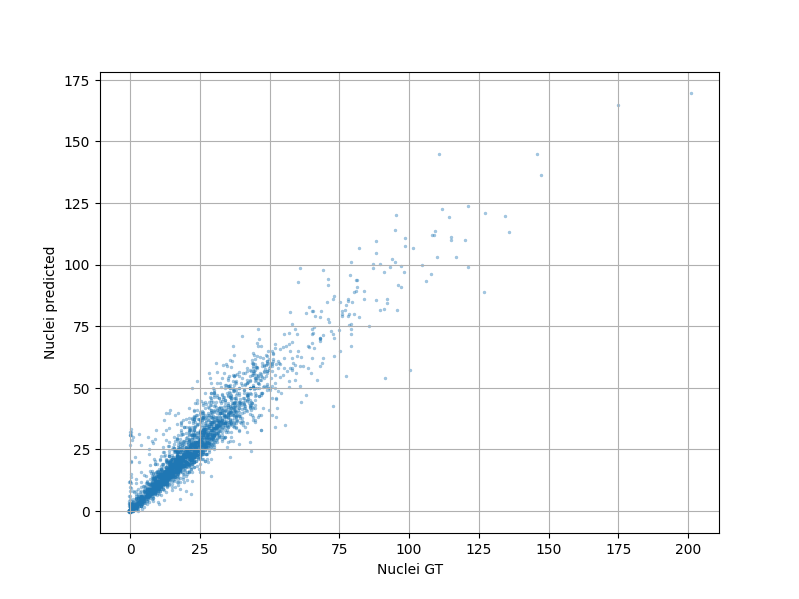
\includegraphics[width=\linewidth]{imgs/Diffusion_graphics_RGB.png}
    \caption*{RGB} % usa \caption* per didascalia senza numerazione
\end{minipage}
\hspace{0.5cm}
\begin{minipage}{0.45\textwidth}
    \centering
    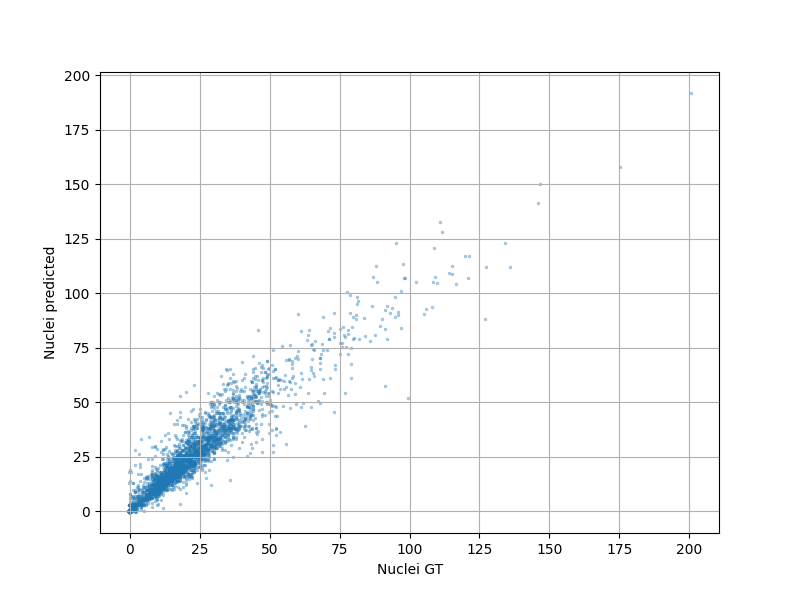
\includegraphics[width=\linewidth]{imgs/grafo_diffusione_HE.png}
    \caption*{H\&E}
\end{minipage}

\vspace{0.5cm}

\begin{minipage}{0.45\textwidth}
    \centering
    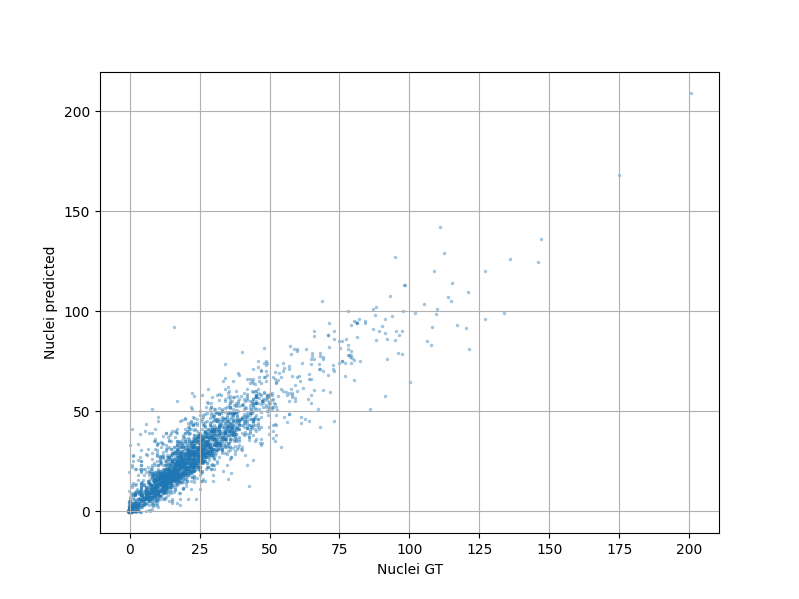
\includegraphics[width=\linewidth]{imgs/diffusion_graph_blu.png}
    \caption*{Blue channel}
\end{minipage}
\hspace{0.5cm}
\begin{minipage}{0.45\textwidth}
    \centering
    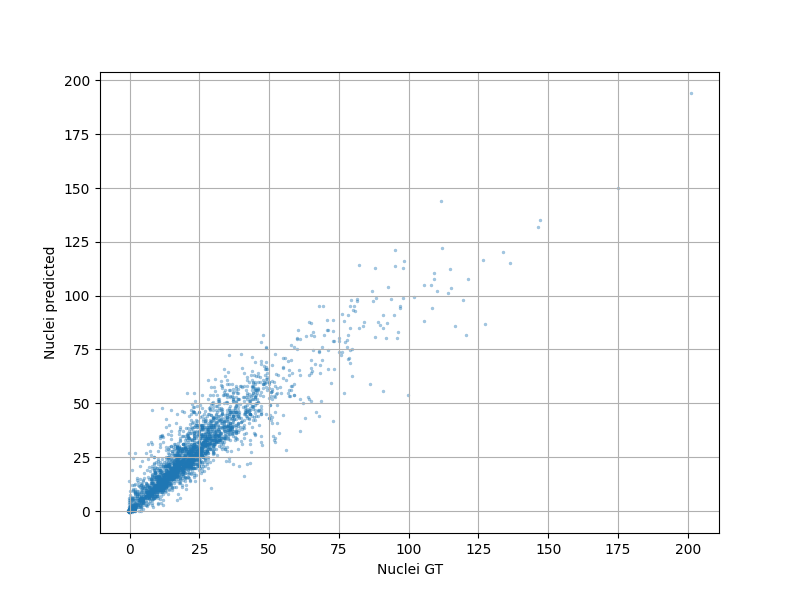
\includegraphics[width=\linewidth]{imgs/Diffusion_graph_gray.png}
    \caption*{Grayscale}
\end{minipage}

\caption{Scatter plots of predicted versus ground-truth nuclei counts for each input modality. Metrics reported in the plot titles include MAE, $R^2$, and $\rho$ (Pearson).}
\label{fig:scatter_counts}
\end{figure}

\subsection{Numerical summary}
Table~\ref{tab:counting_results} reports the quantitative metrics associated with the scatter plots. 
The RGB variant achieves the lowest MAE and the highest correlation scores, followed closely by Hematoxylin. 
The Blue variant shows the weakest performance, while Gray lies in between.

\begin{table}[h]
    \centering
    \caption{Counting performance summary across modalities. $\downarrow$: lower is better, $\uparrow$: higher is better. Best values in \textbf{bold}.}
    \label{tab:counting_results}
    \begin{tabular}{lccc}
        \hline
        \textbf{Input} & \textbf{MAE} $\downarrow$ & \textbf{$R^2$} $\uparrow$ & \textbf{$\rho$} $\uparrow$ \\
        \hline
        RGB         & 4.9 & 0.852 & \textbf{0.948} \\
        Hematoxylin & \textbf{4.7}          & \textbf{0.867}          & 0.948 \\
        Blue        & 6.2          & 0.789          & 0.925 \\
        Gray        & 6.3          & 0.790          & 0.929 \\
        \hline
    \end{tabular}
\end{table}

\noindent\textbf{Discussion.} 
Both scatter plots and quantitative metrics confirm that RGB and Hematoxylin representations are the most effective for nuclei counting. 
Blue channel inputs lead to systematic underestimation in high-density regions, reflected by the lower $R^2$. 
Grayscale remains competitive but with higher error variance.

\section{Category-wise analysis}
To evaluate whether performance depends on nuclear morphology, we categorized the test set into four groups based on nuclear size (small vs.~large) and density (high vs.~low). 
Figure~\ref{fig:boxplot_categories} shows the distribution of counting errors across these categories for each preprocessing modality. 
Negative errors indicate underestimation, while positive values correspond to overestimation.

\begin{figure}[h]
    \centering
    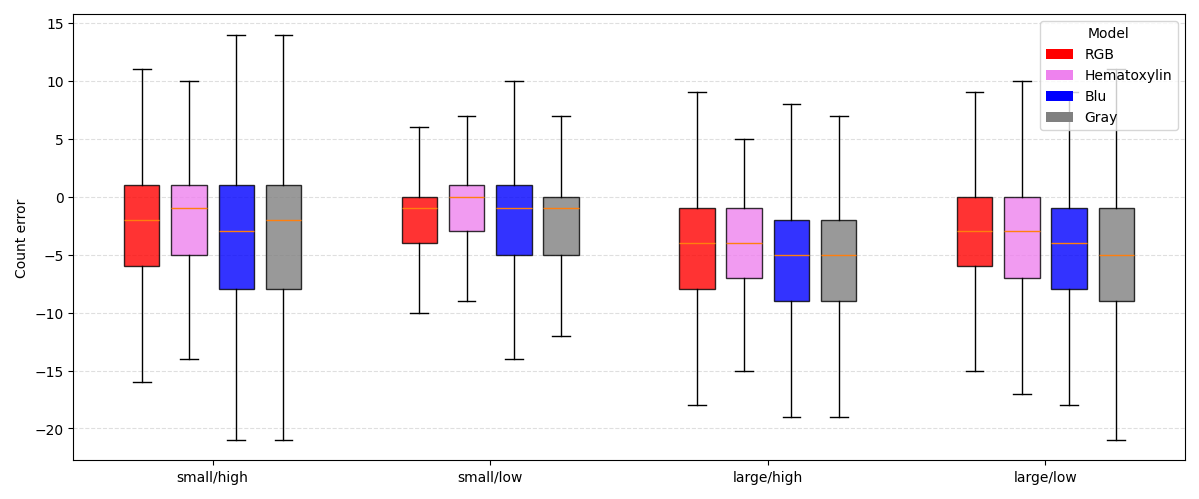
\includegraphics[width=\textwidth]{imgs/boxplot.png}
    \caption{Distribution of counting errors by category. Categories are defined by nuclear size (small/large) and density (high/low). Each boxplot corresponds to one preprocessing modality (RGB, H\&E, Blue, Gray).}
    \label{fig:boxplot_categories}
\end{figure}

\noindent\textbf{Discussion.} 
Errors are more pronounced in the \textbf{large/high-density} category, confirming the difficulty of segmenting overlapping nuclei. 
The Blue variant consistently underestimates across all groups, while RGB and Hematoxylin maintain smaller median errors. 
Gray shows intermediate results but with wider error dispersion, especially in the \textbf{large/low-density} category. 
This analysis highlights that color information not only enhances segmentation but also improves robustness in nuclei counting under challenging conditions.
\section{Qualitative analysis}
\label{sec:qualitative}

Quantitative metrics provide an overall view of performance, but they do not fully capture the visual behaviour of different input modalities. To address this, we complement our evaluation with a qualitative analysis focused on visual inspection of model predictions.\\
We therefore complement the analysis with a qualitative study organised by \emph{difficulty level} (best / typical / hard).. 
For each selected case we report (i) visual outputs for all modalities (\emph{RGB}, \emph{Hematoxylin}, \emph{Blue}, \emph{Gray}) after post-processing and (ii) the associated per-image metrics:
\[
\text{MAE} = |\hat{n}-n|,\quad
\text{AJI},\quad
\text{DICE2},\quad
\text{DQ},\quad
\text{SQ},\quad
\text{PQ}=\text{DQ}\times\text{SQ}.
\]
Here, MAE is the absolute counting error; AJI and DICE2 are instance-level overlaps; DQ and SQ factorise panoptic quality (\S\ref{sec:metrics}).\\
We present the results on images excluded from training, used solely for qualitative evaluation.

\subsection{Case selection and ranking}
We define three difficulty levels using the \textbf{RGB} model as reference (selection is then fixed and reused across modalities):
\begin{itemize}
  \item \textbf{Best}: highest PQ (tie-break by AJI), with MAE close to $0$.
  \item \textbf{Typical}: PQ close to the median of the test-set distribution and moderate MAE.
  \item \textbf{Hard}: lowest PQ (tie-break by AJI), and large MAE (severe under/over-count).
\end{itemize}
This ranking isolates visual patterns behind high/low performance and ensures comparability between modalities.

% ---------- OPTIONAL MACROS FOR INLINE MINI-TABLES ----------
% (decommenta se vuoi usare la mini-tabella sotto ogni immagine)
% \newcommand{\minimetrics}[6]{%
% \vspace{2pt}\footnotesize
% \begin{tabular}{@{}l@{\,}l@{}}
% MAE & #1\\
% AJI & #2\\
% DICE2 & #3\\
% DQ & #4\\
% SQ & #5\\
% PQ & #6\\
% \end{tabular}
% }

\subsection{Best case}
Tabel~\ref{tab:best_metrics} presents the cover percentage and the count error for the sample image shown in figure~\ref{fig:qual_best} that is a representative \emph{best} sample. All modalities delineate nuclei well; \emph{RGB} and \emph{Hematoxylin} exhibit the cleanest borders and the smallest counting error.

\begin{figure}[!htbp]
\centering

\begin{subfigure}{0.48\textwidth}
  \centering
  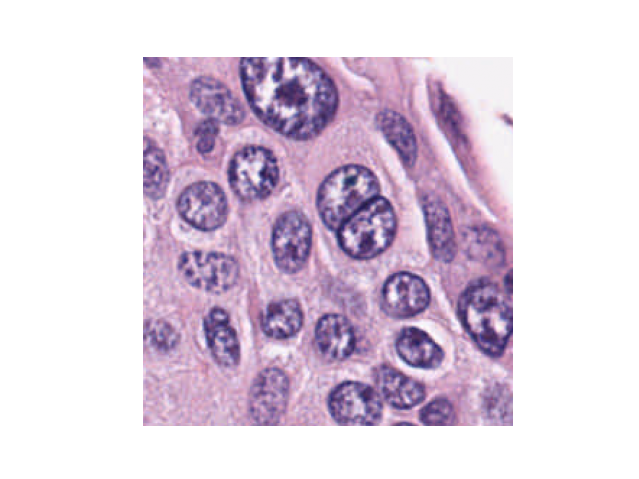
\includegraphics[width=\linewidth]{imgs/qualitative/best/RGB/img.png}
  \caption{Source Image}
\end{subfigure}\hfill
\begin{subfigure}{0.48\textwidth}
  \centering
  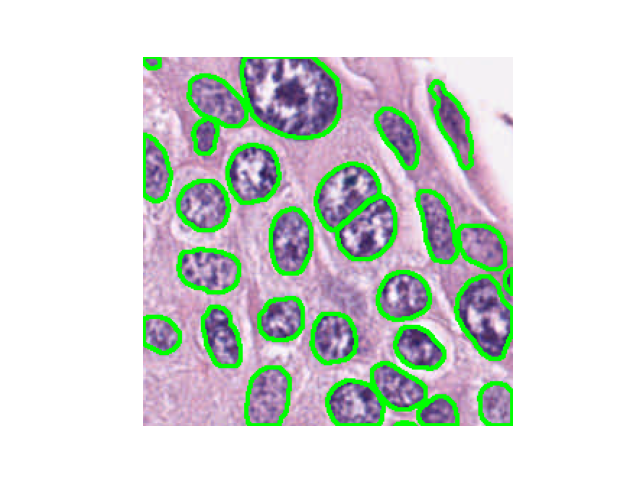
\includegraphics[width=\linewidth]{imgs/qualitative/best/contour_img.png}
  \caption{Ground Truth}
\end{subfigure}

\begin{subfigure}{0.48\textwidth}
  \centering
  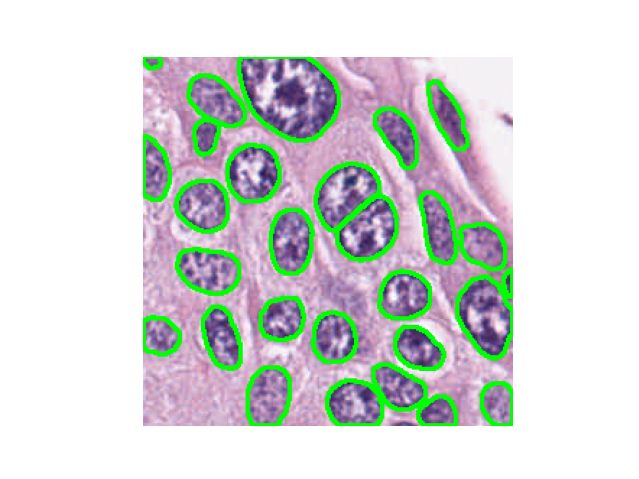
\includegraphics[width=\linewidth]{imgs/qualitative/best/RGB/contour_img.png}
  \caption{RGB}
\end{subfigure}\hfill
\begin{subfigure}{0.48\textwidth}
  \centering
  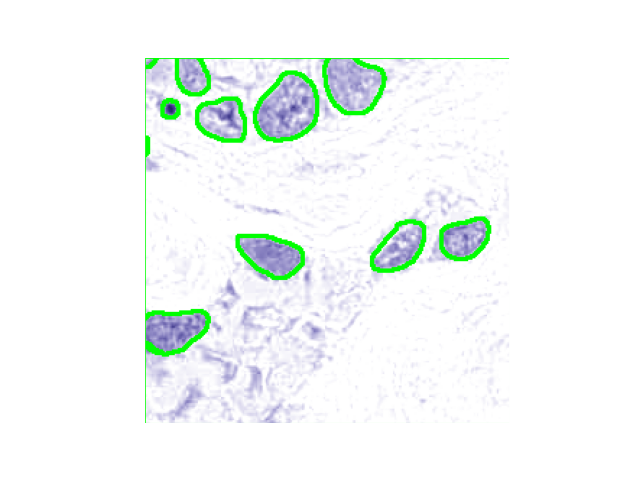
\includegraphics[width=\linewidth]{imgs/qualitative/best/HE/contour_img.png}
  \caption{H\&E}
\end{subfigure}

\begin{subfigure}{0.48\textwidth}
  \centering
  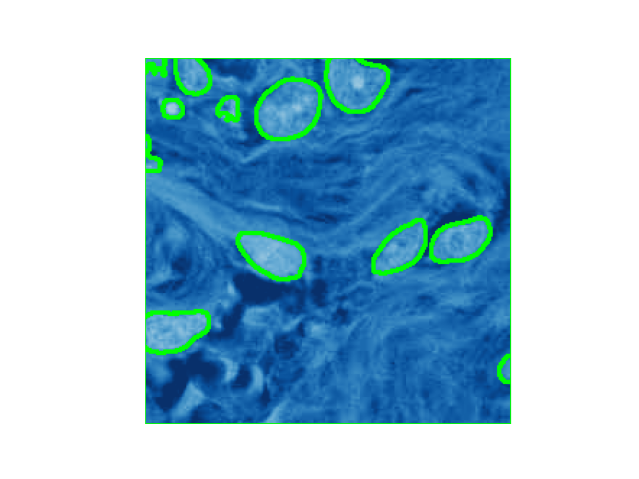
\includegraphics[width=\linewidth]{imgs/qualitative/best/Blu/contour_img.png}
  \caption{Blue}
\end{subfigure}\hfill
\begin{subfigure}{0.48\textwidth}
  \centering
  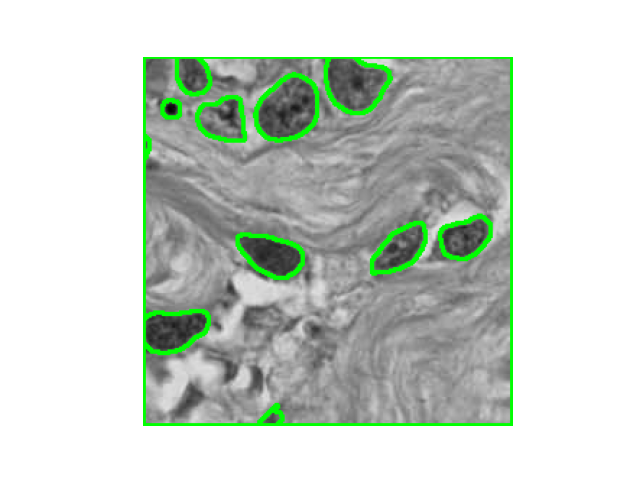
\includegraphics[width=\linewidth]{imgs/qualitative/best/Gray/contour_img.png}
  \caption{Gray}
\end{subfigure}

\caption{Qualitative visualization of nuclei segmentation for the best case. 
Contours of predicted nuclei are shown in green. 
(b) Ground-truth segmentation. 
(c--f) Predictions from models trained on different input modalities: (c) RGB, (d) Hematoxylin, (e) Blue, and (f) Grayscale.}
\label{fig:qual_best}
\end{figure}
\begin{table}[ht]
\centering
\caption{Per-image metrics for the \textbf{best} case across input modalities (RGB, Hematoxylin, Blue, Grayscale). }
\label{tab:best_metrics}
\begin{tabular}{lcccccc}
\toprule
Modality & MAE & AJI & DICE2 & DQ & SQ & PQ \\
\midrule
RGB  & \textbf{0} & \textbf{0.726} & 0.841 & \textbf{0.999} & 0.726 & \textbf{0.726} \\
H\&E & 1 & 0.724 & \textbf{0.855} & 0.947 & \textbf{0.747} & 0.708 \\
Blue & 4 & 0.617 & 0.796 & 0.636 & 0.697 & 0.443 \\
Gray & 1 & 0.712 & 0.850 & 0.947 & 0.725 & 0.686 \\
\bottomrule
\end{tabular}
\end{table}
The predicted values from the segmentation models are remarkably close to the segmentation generated from the ground truth data \ref{fig:qual_best}b. 
\subsection{Typical case}
In the \emph{typical} case (Fig.~\ref{fig:qual_typical}), borders remain well defined but touching nuclei start to merge in \emph{Blue} and \emph{Gray}, increasing MAE. \emph{RGB} and \emph{Hematoxylin} keep higher DQ and AJI.

\begin{figure}[!htbp]
\centering

\begin{subfigure}{0.48\textwidth}
  \centering
  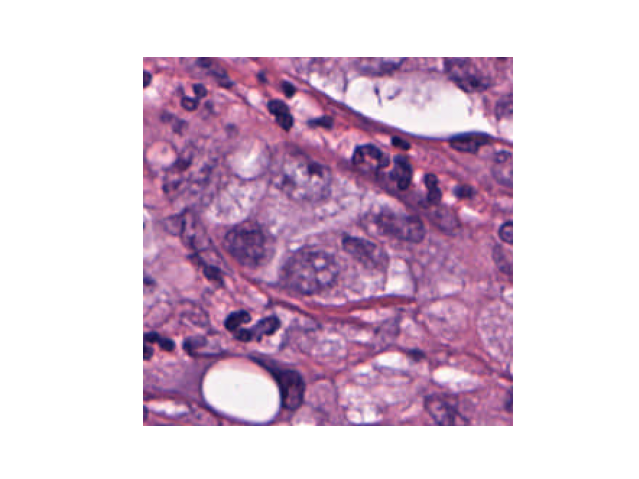
\includegraphics[width=\linewidth]{imgs/qualitative/medium/RGB/img.png}
  \caption{Source Image}
\end{subfigure}\hfill
\begin{subfigure}{0.48\textwidth}
  \centering
  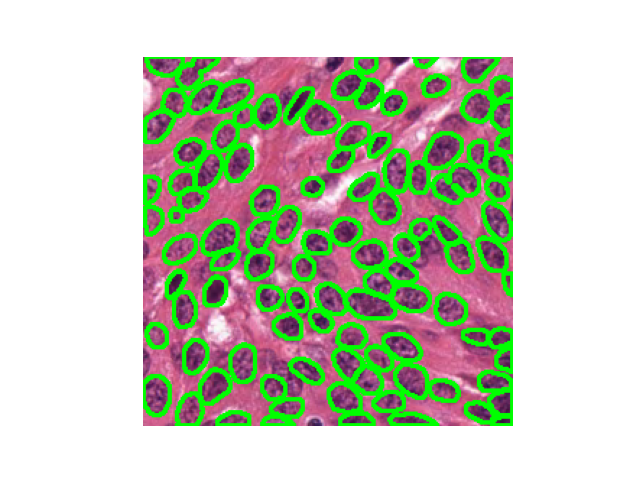
\includegraphics[width=\linewidth]{imgs/qualitative/medium/contour_img.png}
  \caption{Ground Truth}
\end{subfigure}

\begin{subfigure}{0.48\textwidth}
  \centering
  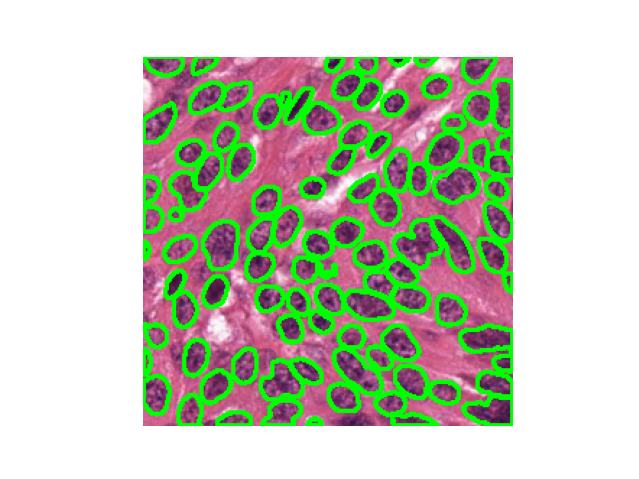
\includegraphics[width=\linewidth]{imgs/qualitative/medium/RGB/contour_img.png}
  \caption{RGB}
\end{subfigure}\hfill
\begin{subfigure}{0.48\textwidth}
  \centering
  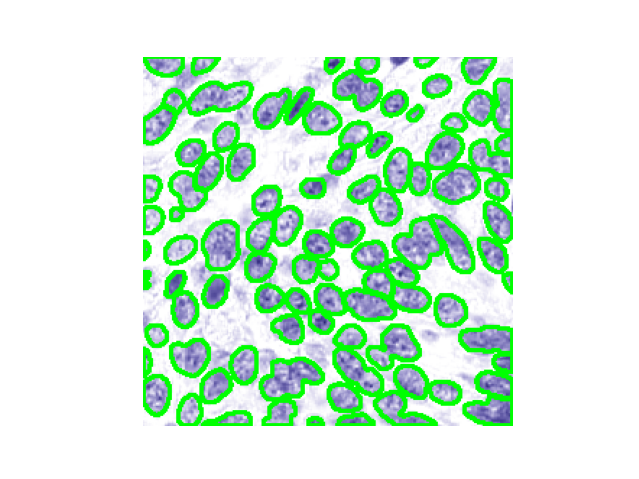
\includegraphics[width=\linewidth]{imgs/qualitative/medium/HE/contour_img.png}
  \caption{H\&E}
\end{subfigure}

\begin{subfigure}{0.48\textwidth}
  \centering
  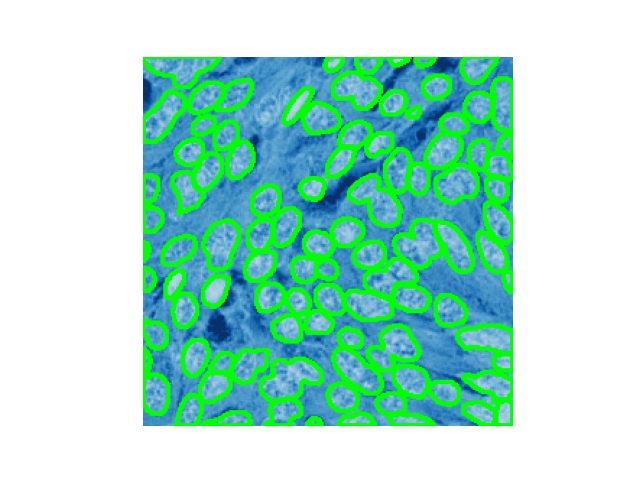
\includegraphics[width=\linewidth]{imgs/qualitative/medium/Blu/contour_img.png}
  \caption{Blue}
\end{subfigure}\hfill
\begin{subfigure}{0.48\textwidth}
  \centering
  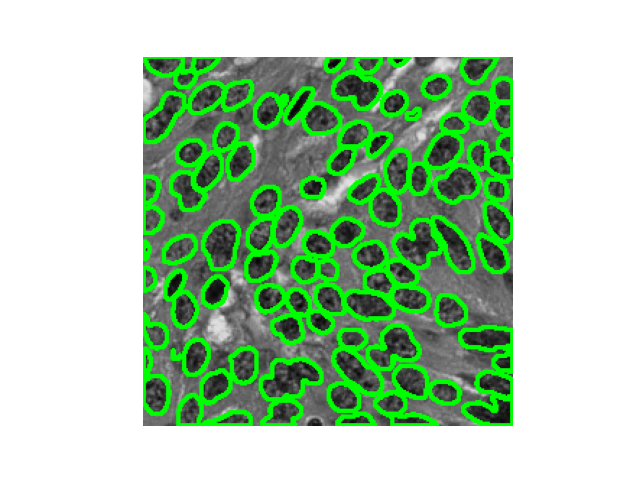
\includegraphics[width=\linewidth]{imgs/qualitative/medium/Gray/contour_img.png}
  \caption{Gray}
\end{subfigure}

\caption{Qualitative visualization of nuclei segmentation for the typical case. 
Contours of predicted nuclei are shown in green. 
(b) Ground-truth segmentation. 
(c--f) Predictions from models trained on different input modalities: (c) RGB, (d) Hematoxylin, (e) Blue, and (f) Grayscale.}
\label{fig:qual_typical}
\end{figure}
\begin{table}[ht]
\centering
\caption{Per-image metrics for the \textbf{typical} case across input modalities (RGB, Hematoxylin, Blue, Grayscale). }
\label{tab:typical_metrics}
\begin{tabular}{lcccccc}
\toprule
Modality & MAE & AJI & DICE2 & DQ & SQ & PQ \\
\midrule
RGB  & \textbf{5} & \textbf{0.567} & \textbf{0.667} & \textbf{0.639} & \textbf{0.730} & \textbf{0.467} \\
H\&E & 4 & 0.560 & 0.645 & 0.621 & 0.719 & 0.447 \\
Blue & 3 & 0.505 & 0.623 & 0.597 & 0.675 & 0.403 \\
Gray & 5 & 0.576 & 0.674 & 0.639 & 0.709 & 0.454 \\
\bottomrule
\end{tabular}
\end{table}
\subsection{Hard case}
The \emph{hard} case (Fig.~\ref{fig:qual_hard}) features overlapping/weakly stained nuclei. All modalities deteriorate, but \emph{RGB}/\emph{Hematoxylin} retain higher DQ (more detections) and AJI than \emph{Blue}, which shows under-segmentation (high MAE).

\begin{figure}[!htbp]
\centering
\begin{subfigure}{0.48\textwidth}
  \centering
  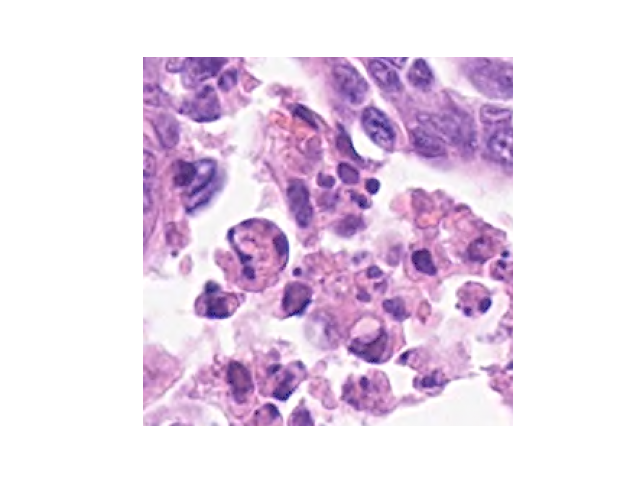
\includegraphics[width=\linewidth]{imgs/qualitative/worst/RGB/img.png}
  \caption{Source Image}
\end{subfigure}\hfill
\begin{subfigure}{0.48\textwidth}
  \centering
  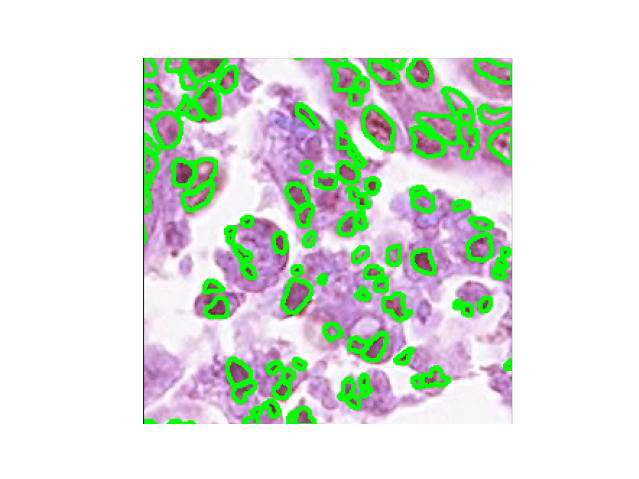
\includegraphics[width=\linewidth]{imgs/qualitative/worst/contour_img.png}
  \caption{Ground Truth}
\end{subfigure}

\begin{subfigure}{0.48\textwidth}
  \centering
  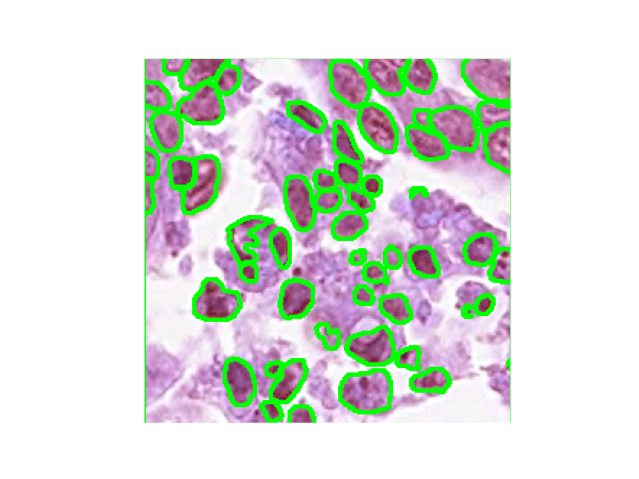
\includegraphics[width=\linewidth]{imgs/qualitative/worst/RGB/contour_img.png}
  \caption{RGB}
\end{subfigure}\hfill
\begin{subfigure}{0.48\textwidth}
  \centering
  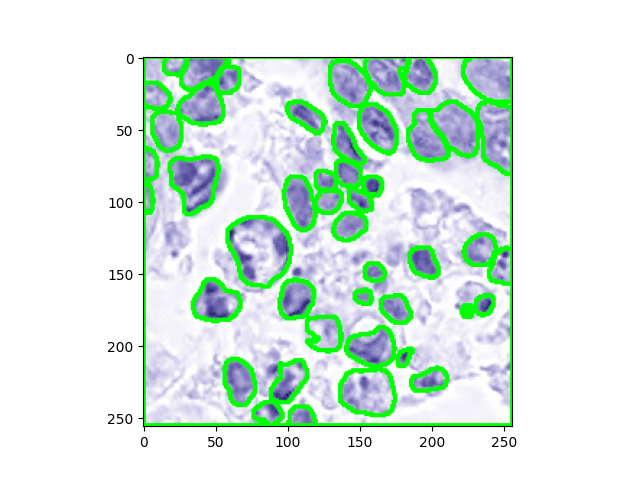
\includegraphics[width=\linewidth]{imgs/qualitative/worst/HE/contour_img.png}
  \caption{H\&E}
\end{subfigure}

\begin{subfigure}{0.48\textwidth}
  \centering
  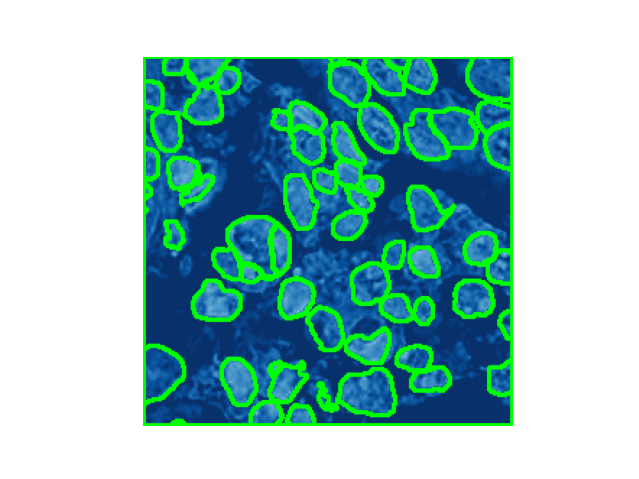
\includegraphics[width=\linewidth]{imgs/qualitative/worst/Blu/contour_img.png}
  \caption{Blue}
\end{subfigure}\hfill
\begin{subfigure}{0.48\textwidth}
  \centering
  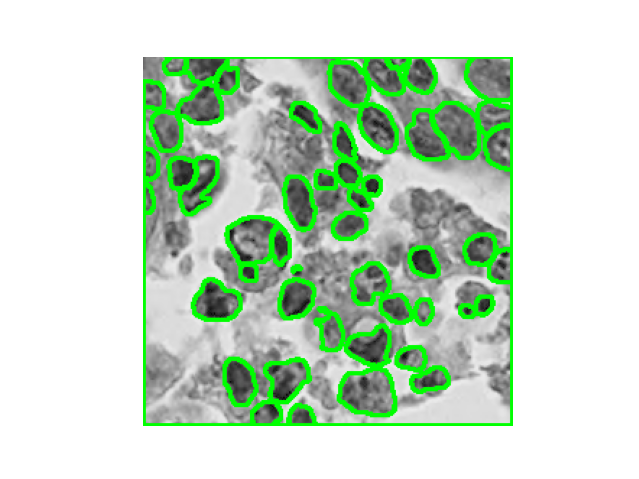
\includegraphics[width=\linewidth]{imgs/qualitative/worst/Gray/contour_img.png}
  \caption{Gray}
\end{subfigure}

\caption{Qualitative visualization of nuclei segmentation for the worst/hard case. 
Contours of predicted nuclei are shown in green. 
(b) Ground-truth segmentation. 
(c--f) Predictions from models trained on different input modalities: (c) RGB, (d) Hematoxylin, (e) Blue, and (f) Grayscale.}
\label{fig:qual_hard}
\end{figure}
\begin{table}[ht]
\centering
\caption{Per-image metrics for the hard case across input modalities (RGB, Hematoxylin, Blue, Grayscale). }
\label{tab:worst_metrics}
\begin{tabular}{lcccccc}
\toprule
Modality & MAE & AJI & DICE2 & DQ & SQ & PQ \\
\midrule
RGB  & 43 & \textbf{0.265} & \textbf{0.386} & \textbf{0.292} & 0.630 & 0.184 \\
H\&E & 53 & 0.208 & 0.324 & 0.272 & 0.630 & 0.171 \\
Blue & \textbf{37} & 0.235 & 0.356 & 0.257 & 0.635 & 0.163 \\
Gray & 46 & 0.237 & 0.355 & 0.285 & \textbf{0.647} & \textbf{0.185} \\
\bottomrule
\end{tabular}
\end{table}
\subsection{Discussion}
The results discused in this chapter can be directly related to figure~\ref{fig:boxplot_categories}, which provides a visual summary of the observed trends. The qualitative study reveals consistent patterns across modalities once cases are stratified by morphology and difficulty:

\paragraph{Best (Large / Low-density).}
Patches with large nuclei and ample inter-nuclear spacing are the easiest setting. All modalities delineate instances well, with \textbf{RGB} and \textbf{Hematoxylin} yielding near-perfect overlays, the highest AJI/DICE2 and PQ, and MAE $\approx 0$. In these conditions, boundaries are well contrasted and the watershed separation is rarely needed, so segmentation quality (SQ) saturates and detection quality (DQ) approaches~1.

\paragraph{Typical (Small / Low-density).}
When nuclei are \emph{small} but the scene remains relatively sparse, performance drops moderately. \textbf{RGB} and \textbf{Hematoxylin} retain competitive AJI/DICE2 and DQ, while \textbf{Gray} stays close and \textbf{Blue} shows the first signs of under-segmentation (merging of nearby instances). Counting errors (MAE) increase mainly due to missed small detections rather than gross mask failures, which is reflected by a larger hit on DQ than on SQ.

\paragraph{Hard (Small / High-density).}
The most challenging regime combines small nuclei with crowding/overlap. Here all modalities degrade, but \textbf{RGB}/\textbf{Hematoxylin} remain relatively more reliable than \textbf{Blue}/\textbf{Gray}. Errors are dominated by \emph{under-segmentation} and \emph{missed detections}: DQ drops sharply and AJI/DICE2 fall due to instance mergers, while SQ remains comparatively less affected (masks are reasonable where detections happen). This mismatch explains the high MAE despite moderate SQ.

\paragraph{Modality-wise summary.}
Across all difficulty levels, \textbf{RGB} and \textbf{Hematoxylin} systematically achieve higher AJI/DICE2 and PQ with lower MAE, indicating a better balance between detection (DQ) and mask fidelity (SQ). \textbf{Blue} is the least robust in crowded fields (low DQ, larger MAE) and \textbf{Gray} is competitive in simpler scenes but less stable in small/high-density regimes.



\chapter{Conclusion}
\paragraph{Takeaways for practice.}
(1) When tissue appearance permits, prefer \textbf{RGB} or \textbf{Hematoxylin} inputs to maximize instance recall and counting accuracy.  
(2) The primary failure mode in difficult scenes is detection/instance separation (DQ), not mask sharpness (SQ); improving boundary cues and separation priors (e.g., stronger distance-map weighting or learned boundary heads) is likely to yield the biggest gains.  
(3) Since difficulty is tightly coupled to \emph{size} and \emph{density}, targeted augmentation (small objects, clustered placements) and curriculum-style hard-mining may further reduce MAE in the Small/High-density regime.

Overall, the qualitative evidence aligns with quantitative trends: color information (RGB/Hematoxylin) improves robustness, especially for instance recall in crowded regions, while morphology (small size, high density) is the dominant driver of failure through missed detections and merged instances.
%% Fine dei capitoli normali, inizio dei capitoli-appendice (opzionali)
\appendix

%\part{Appendici}

\chapter{Titolo della prima appendice}
Sed purus libero, vestibulum ut nibh vitae, mollis ultricies augue. Pellentesque velit libero, tempor sed pulvinar non, fermentum eu leo. Duis posuere eleifend nulla eget sagittis. Nam laoreet accumsan rutrum. Interdum et malesuada fames ac ante ipsum primis in faucibus. Curabitur eget libero quis leo porttitor vehicula eget nec odio. Proin euismod interdum ligula non ultricies. Maecenas sit amet accumsan sapien.

%% Parte conclusiva del documento; tipicamente per riassunto, bibliografia e/o indice analitico.
\backmatter

%% Riassunto (opzionale)
%\summary
%Maecenas tempor elit sed arcu commodo, dapibus sagittis leo egestas. Praesent at ultrices urna. Integer et nibh in augue mollis facilisis sit amet eget magna. Fusce at porttitor sapien. Phasellus imperdiet, felis et molestie vulputate, mauris sapien tincidunt justo, in lacinia velit nisi nec ipsum. Duis elementum pharetra lorem, ut pellentesque nulla congue et. Sed eu venenatis tellus, pharetra cursus felis. Sed et luctus nunc. Aenean commodo, neque a aliquam bibendum, mauris augue fringilla justo, et scelerisque odio mi sit amet diam. Nulla at placerat nibh, nec rutrum urna. Donec ut egestas magna. Aliquam erat volutpat. Phasellus vestibulum justo sed purus mattis, vitae lacinia magna viverra. Nulla rutrum diam dui, vel semper mi mattis ac. Vestibulum ante ipsum primis in faucibus orci luctus et ultrices posuere cubilia Curae; Donec id vestibulum lectus, eget tristique est.

%% Bibliografia (praticamente obbligatoria)
\bibliographystyle{plain_\languagename}%% Carica l'omonimo file .bst, dove \languagename è la lingua attiva.
%% Nel caso in cui si usi un file .bib (consigliato)
\bibliography{thud}
%% Nel caso di bibliografia manuale, usare l'environment thebibliography.
%% Per l'indice analitico, usare il pacchetto makeidx (o analogo).

\end{document}

--- Istruzioni per l'aggiunta di nuove lingue ---
Per ogni nuova lingua utilizzata aggiungere nel preambolo il seguente spezzone:
    \addto\captionsitalian{%
        \def\abstractname{Sommario}%
        \def\acknowledgementsname{Ringraziamenti}%
        \def\authorcontactsname{Contatti dell'autore}%
        \def\candidatename{Candidato}%
        \def\chairname{Direttore}%
        \def\conclusionsname{Conclusioni}%
        \def\cosupervisorname{Co-relatore}%
        \def\cosupervisorsname{Co-relatori}%
        \def\cyclename{Ciclo}%
        \def\datename{Anno accademico}%
        \def\indexname{Indice analitico}%
        \def\institutecontactsname{Contatti dell'Istituto}%
        \def\introductionname{Introduzione}%
        \def\prefacename{Prefazione}%
        \def\reviewername{Controrelatore}%
        \def\reviewersname{Controrelatori}%
        %% Anno accademico
        \def\shortdatename{A.A.}%
        \def\summaryname{Riassunto}%
        \def\supervisorname{Relatore}%
        \def\supervisorsname{Relatori}%
        \def\thesisname{Tesi di \expandafter\ifcase\csname thud@target\endcsname Laurea\or Laurea Triennale\or Dottorato\fi}%
        \def\tutorname{Tutor aziendale}%
        \def\tutorsname{Tutor aziendali}%
    }
